\documentclass[12pt]{article}

\usepackage{sbc-template}
\usepackage{graphicx,url}
\usepackage[utf8]{inputenc}
\usepackage[T1]{fontenc}
\usepackage[brazilian]{babel}
\usepackage{booktabs,array,tabularx}
\usepackage{xcolor}
\usepackage{tikz}
\usetikzlibrary{positioning,shapes.geometric,arrows.meta,fit,calc,patterns,backgrounds}
\usepackage{pgfplots}
\pgfplotsset{compat=1.17}

\sloppy

% Estilos comuns das figuras (TikZ)
\tikzset{
  caixa/.style={draw, rounded corners=2pt, align=center, font=\footnotesize,
    inner sep=3pt, fill=white},
  cinza/.style={fill=gray!15},
  seta/.style={-{Stealth[length=2.2mm]}, thick},
}

% Citacoes: o texto aprovado usa o formato "[Autor ano]" e "Autor (ano)";
% \nocite registra a entrada na bibliografia.
\newcommand{\cit}[2]{[#1]\nocite{#2}}
\newcommand{\citn}[2]{#1\nocite{#2}}


\title{Masquerade em GOOSE: por que IDS de estado, autenticação por mensagem (HMAC) e 802.1X, isoladamente, não bastam\\[6pt]{\large\mdseries Avaliação experimental em testbed emulado, com quadros GOOSE derivados de um único quadro real capturado de um relé SEL-351}}

\author{Lucas Mota\inst{1}, Matheus\inst{1}, Youri\inst{1}}

\address{Universidade Federal do Sul e Sudeste do Par\'a (Unifesspa)}

\begin{document}

\maketitle

\begin{abstract}
GOOSE masquerade forges frames consistent with the protocol's state. We evaluate, with a cloned (C1) or the attacker's own (C2) MAC, a passive state-based IDS, simulated per-message authentication (HMAC), and 802.1X with EAP-TLS and a certificate-MAC binding. Frames derive from a single frame captured from an SEL-351 relay, combining an offline campaign (100 repetitions per scenario) with GNS3 executions (one per scenario). The IDS detected C2 but not C1; HMAC verification rejected C1 without the key, but not once the key leaked; 802.1X blocked invalid credentials and MAC mismatches, but not an authenticated node using its own MAC. In the evaluated scenarios the layers complemented each other, without proving full protection.

\noindent\textbf{Keywords} IEC 61850; GOOSE; masquerade; intrusion detection; IEEE 802.1X.
\end{abstract}

\begin{resumo}
O masquerade em GOOSE forja quadros coerentes com o estado do protocolo. Avaliamos, com MAC clonado (C1) e próprio (C2), um IDS de estado passivo, autenticação por mensagem simulada (HMAC) e controle 802.1X com EAP-TLS e vínculo entre certificado e MAC. Os quadros derivam de um único quadro capturado de um relé SEL-351; combinamos uma campanha \emph{offline} (100 repetições por cenário) e o GNS3 (uma execução por cenário). O IDS detectou C2, mas não C1; a verificação HMAC rejeitou C1 sem a chave, mas não quando ela foi vazada; o 802.1X barrou credenciais inválidas e MAC divergente, mas não um nó autenticado com o próprio MAC. Nos cenários avaliados, as camadas se complementaram, sem comprovar proteção completa.

\noindent\textbf{Palavras-chave} IEC 61850; GOOSE; masquerade; detecção de intrusão; IEEE 802.1X.
\end{resumo}

\section{Introdução}\label{sec:1}

A digitalização das subestações elétricas, orientada pela norma IEC 61850, substituiu a fiação rígida entre os dispositivos de proteção e controle por redes Ethernet \cit{Herath et al. 2025}{herath2025evaluation} e, com isso, ampliou a superfície de ataque do setor elétrico \cit{Oliveira e Gurjão 2025; de Oliveira et al. 2023}{oliveira2025analisador,oliveira2023ataques}. Nesse modelo, as mensagens GOOSE (\emph{Generic Object Oriented Substation Event}) levam entre os IEDs eventos de proteção, como a ordem de abertura de um disjuntor. Em razão dos requisitos de baixa latência, elas são mapeadas diretamente sobre a camada de enlace, em multicast e no modelo publicador-assinante \cit{Herath et al. 2025; de Oliveira et al. 2023}{herath2025evaluation,oliveira2023ataques} e, em sua forma básica, sem as extensões de segurança da IEC 62351-6, não oferecem nenhum mecanismo de segurança embutido \cit{Herath et al. 2025}{herath2025evaluation}. Um adversário que obtenha acesso à rede local da subestação pode, assim, atacar esse tráfego \cit{Herath et al. 2025}{herath2025evaluation}.

Entre os ataques ao GOOSE, o \emph{masquerade} (mascaramento) se distingue porque o quadro forjado pode respeitar as regras de evolução de estado do protocolo. Nos trabalhos analisados, a atualidade de uma mensagem é inferida pela evolução de \texttt{stNum}, que cresce a cada mudança de estado, e de \texttt{sqNum}, que cresce a cada retransmissão e volta a zero quando o estado muda \cit{Herath et al. 2025; Conceição Alberto et al. 2026}{herath2025evaluation,alberto2026gooseidrs}. Em experimentos de \emph{hardware-in-the-loop}, \citn{Conceição Alberto et al. (2026)}{alberto2026gooseidrs} reportam que um quadro forjado com \texttt{stNum} igual ao do último quadro legítimo mais um e \texttt{sqNum} zerado foi aceito pelos assinantes, e que as atualizações legítimas seguintes, com \texttt{stNum} menor, foram rejeitadas. Esses autores sintetizam ainda que replay, envenenamento e flooding não provocaram má operação observável em condições realistas, ao passo que o masquerade a provocou de forma consistente. De Oliveira et al. (2023), porém, descrevem efeitos de replay e de negação de serviço em seu cenário, além da abertura de um disjuntor simulado por um masquerade construído a partir de mensagens de um IED real.

A literatura analisada responde a esse risco com três famílias de defesa. Sistemas de detecção de intrusão (IDS) verificam a semântica do protocolo, por regras sobre \texttt{stNum}, \texttt{sqNum} e temporização \cit{Herath et al. 2025}{herath2025evaluation} ou por aprendizado de máquina \cit{Conceição Alberto et al. 2026; Moore 2026}{alberto2026gooseidrs,moore2026anomaly}. A autenticação por mensagem, prevista na IEC 62351-6 \cit{IEC 2020}{iec62351-6}, anexa a cada quadro um código de autenticação calculado com uma chave compartilhada \cit{Herath et al. 2025; Hussain et al. 2023}{herath2025evaluation,hussain2023hybrid}. \emph{Switches} definidos por software, por fim, bloqueiam a porta do dispositivo malicioso, mas depois da detecção \cit{Girdhar et al. 2024}{girdhar2024sdn}. Há trabalhos que combinam as duas primeiras famílias \cit{Herath et al. 2025}{herath2025evaluation}, e a comparação detalhada é apresentada na Seção~\ref{sec:2}.

Essas avaliações partem, porém, de hipóteses que podem não se sustentar. No trabalho analisado que combina autenticação e detecção, a verificação de MAC é avaliada contra quadros adulterados, e a possibilidade de comprometimento da chave não é tratada \cit{Herath et al. 2025}{herath2025evaluation}; em outro, o comprometimento de dispositivos e o acesso a chaves criptográficas são excluídos do modelo de ameaças \cit{Conceição Alberto et al. 2026}{alberto2026gooseidrs}. A distribuição segura de chaves compartilhadas é, aliás, apontada como um desafio \cit{Hussain et al. 2023}{hussain2023hybrid}. Também não identificamos, nos trabalhos analisados, a avaliação de um controle de acesso à porta que impeça a entrada do atacante na rede, como o IEEE 802.1X \cit{IEEE 2020}{ieee8021x} com EAP-TLS; o bloqueio de porta de \citn{Girdhar et al. (2024)}{girdhar2024sdn} ocorre depois da detecção do ataque. Por fim, o endereço MAC de origem do quadro forjado, que pode ser o do próprio atacante (C2) ou clonado do publicador legítimo (C1), não é tratado como variável experimental nesses trabalhos; \citn{Moore (2026)}{moore2026anomaly} descreve o masquerade como falsificação do MAC de origem, mas descarta os campos de MAC, entre outras colunas de alta cardinalidade, do conjunto de atributos. Falta, portanto, nos trabalhos analisados, uma avaliação experimental da interação entre detecção, autenticação e controle de acesso diante do masquerade, sobretudo quando a chave é comprometida e quando o MAC de origem é clonado.

Este trabalho se propõe a endereçar essa lacuna. A pergunta de pesquisa é: diante do masquerade em GOOSE com MAC clonado (C1) ou próprio (C2), o que cobrem o IDS de estado (detecção), a autenticação por mensagem (HMAC) e o controle de acesso 802.1X (identidade de rede vinculada ao MAC); onde cada um falha isoladamente, inclusive com a chave comprometida; e como se compensam? O objetivo geral é avaliar experimentalmente essa interação em um \emph{testbed} emulado, com quadros GOOSE derivados de um quadro real capturado de um relé SEL-351.

Duas delimitações orientam a leitura. A autenticação avaliada é uma simulação baseada em HMAC, que representa a ideia da IEC 62351-6 sem implementar o mecanismo normativo. E o IDS é passivo, pois emite alertas em vez de descartar quadros, de modo que seus resultados não se comparam à mitigação em linha nem ao desempenho de abordagens de aprendizado de máquina. Os detalhes estão nas Seções~\ref{sec:4} e \ref{sec:5}.

As contribuições são: (i) a caracterização experimental do ponto cego de um IDS de estado diante do masquerade com MAC clonado (C1), em contraste com a detecção do masquerade com MAC próprio (C2); (ii) a avaliação da autenticação por mensagem simulada, com e sem a chave em poder do atacante, que delimita o ganho que ela traz e onde deixa de proteger; (iii) a implementação e a validação, em \emph{testbed} emulado, de um controle de acesso 802.1X real com EAP-TLS, com vínculo entre o certificado de cada nó e o seu endereço MAC, a partir de um inventário gerado no mesmo fluxo que produz a topologia a partir do arquivo SCD; e (iv) uma análise por cenário e por camada que identifica onde cada defesa falha isoladamente e como elas se compensam.

O restante do artigo está organizado assim: a Seção~\ref{sec:2} apresenta a fundamentação, as normas e os trabalhos relacionados; a Seção~\ref{sec:3}, o modelo de ameaças e os casos de uso; a Seção~\ref{sec:4}, o ambiente experimental e a metodologia; a Seção~\ref{sec:5}, as três camadas de defesa e as modificações feitas no \emph{testbed}; a Seção~\ref{sec:6}, os resultados e as análises; a Seção~\ref{sec:7}, a discussão e as limitações; e a Seção~\ref{sec:8}, a conclusão.

\section{Fundamentação e trabalhos relacionados}\label{sec:2}

Esta seção apresenta os elementos necessários para avaliar as três camadas de defesa do trabalho. A Seção~\ref{sec:2.1} descreve o GOOSE e a taxonomia de ataques adotada; a 2.2, as normas e os mecanismos de autenticação e de controle de acesso; a 2.3, os trabalhos relacionados, organizados pelas três camadas; e a 2.4 situa este trabalho em relação ao artigo que o originou.

\subsection{GOOSE, semântica de estado e taxonomia de ataques}\label{sec:2.1}

O GOOSE é um serviço orientado a eventos, definido na IEC 61850-7-2 e mapeado diretamente sobre Ethernet na IEC 61850-8-1: seus quadros são multicast de camada 2, com marcação VLAN e prioridade, no modelo publicador-assinante \cit{Herath et al. 2025}{herath2025evaluation}. Em regime permanente, as mensagens são retransmitidas em intervalo fixo, com \texttt{stNum} constante e \texttt{sqNum} crescente; quando ocorre um evento, o publicador envia uma mensagem com novo \texttt{stNum} e \texttt{sqNum} igual a zero e passa a retransmiti-la em rajada, com intervalos que crescem até o regime permanente \cit{Herath et al. 2025; Conceição Alberto et al. 2026}{herath2025evaluation,alberto2026gooseidrs}. Os assinantes inferem a atualidade de uma mensagem a partir dessa evolução monotônica e de restrições de temporização, como o \texttt{timeAllowedToLive} \cit{Conceição Alberto et al. 2026}{alberto2026gooseidrs}.

Os requisitos de tempo variam conforme a fonte e a classe de mensagem. \citn{Herath et al. (2025)}{herath2025evaluation} citam 3 ms para o GOOSE do tipo 1A; \citn{Conceição Alberto et al. (2026)}{alberto2026gooseidrs}, cerca de 3 ms para as classes de desempenho P2 e P3 da IEC 61850-5; e \citn{Moore (2026)}{moore2026anomaly} adota 4 ms como o tempo de disparo da proteção de distância. Neste trabalho, o valor de 4 ms é usado como critério experimental de viabilidade nas medições de latência (Seção~\ref{sec:6}), e não como requisito normativo, pois não consultamos o texto da IEC 61850-5.

A literatura descreve os ataques ao GOOSE com variações de nomenclatura. \citn{Conceição Alberto et al. (2026)}{alberto2026gooseidrs} listam masquerade ou spoofing, replay, \texttt{stNum} elevado (envenenamento), injeção de mensagens e flooding; \citn{Herath et al. (2025)}{herath2025evaluation}, replay, masquerade, flooding e descarte de pacotes; \citn{Zemanek et al. (2022)}{zemanek2022powerduck}, replay, inserção, suppression e flooding. Este trabalho usa quatro ataques: flooding, replay, masquerade e suppression. A associação do nosso suppression ao envenenamento por \texttt{stNum} elevado de \citn{Conceição Alberto et al. (2026)}{alberto2026gooseidrs} e à classe suppression de \citn{Zemanek et al. (2022)}{zemanek2022powerduck} é uma interpretação da nossa taxonomia, e não uma equivalência estabelecida nesses trabalhos. O descarte de pacotes de \citn{Herath et al. (2025)}{herath2025evaluation} é um ataque distinto, ao encaminhamento, e não é avaliado aqui.

\subsection{Normas e mecanismos de segurança}\label{sec:2.2}

Segundo \citn{Herath et al. (2025)}{herath2025evaluation}, a IEC 62351-6 \cit{IEC 2020}{iec62351-6} recomenda, para o GOOSE, códigos de autenticação de mensagem (MAC) calculados com chaves pré-compartilhadas e anexados ao quadro em campos de extensão, que incluem um vetor de inicialização, o identificador da chave e a tag, com o AES-GMAC-128 como algoritmo principal. Os mesmos autores indicam que a norma recomenda integrar verificações por regras à verificação de MAC, e que a proteção contra replay é tratada em uma etapa adicional, que verifica \texttt{stNum} e \texttt{sqNum}. A distribuição segura das chaves pré-compartilhadas é apontada como um desafio \cit{Hussain et al. 2023}{hussain2023hybrid}.

A IEC 62443-3-3 \cit{IEC 2013}{iec62443-3-3} estabelece requisitos técnicos de segurança para sistemas de controle industrial. O artigo que originou este trabalho a utilizou para verificar a política de senhas dos IEDs \cit{Oliveira e Gurjão 2025}{oliveira2025analisador}; o Oráculo deste projeto, que realiza a auditoria por SSH, avalia ainda credenciais padrão, privilégio da conta, integridade das mensagens GOOSE, segmentação por VLAN e limitação de taxa de conexões. Citamos esses requisitos pelo conteúdo, e não pelo número, porque a correspondência com a numeração da norma ainda não foi verificada contra o texto normativo.

O IEEE 802.1X \cit{IEEE 2020}{ieee8021x} trata do controle de acesso à rede baseado em porta: o dispositivo só tem a porta liberada depois de ser autenticado. Com o EAP-TLS, a autenticação é mútua e baseada em certificados \cit{Simon et al. 2008}{rfc5216}. Segundo o RFC 9190, o servidor deve se autenticar com um certificado e é recomendável que exija também o certificado do par \cit{Preuß Mattsson e Sethi 2022}{rfc9190}. O RFC 5216 define o EAP-TLS, e o RFC 9190 o atualiza para o TLS 1.3, mantendo o RFC 5216 aplicável quando o TLS 1.2 é negociado \cit{Preuß Mattsson e Sethi 2022}{rfc9190}. Em uma medição em ambiente de depuração, fora do GNS3, com \texttt{hostapd} e \texttt{wpa\_\allowbreak{}supplicant} 2.10 e OpenSSL 3.5.7 e a configuração do projeto, a negociação resultou em TLS 1.2; o TLS 1.3 não foi negociado nem quando habilitado explicitamente nas duas pontas, e a causa não foi investigada. Para a configuração medida, o texto aplicável é, portanto, o RFC 5216 (a medição está disponível no repositório do projeto).

A Tabela~\ref{tab:1} relaciona cada ataque à propriedade comprometida e ao que as normas e os trabalhos analisados dizem sobre ele; as observações do nosso \emph{testbed} ficam para a Seção~\ref{sec:6}.

\begin{table}[!t]
\centering
\caption{Ataques, propriedade comprometida e o que dizem as normas e a literatura analisada.}\label{tab:1}
\footnotesize
\begin{tabularx}{\linewidth}{>{\hsize=0.644\hsize\raggedright\arraybackslash}X>{\hsize=0.868\hsize\raggedright\arraybackslash}X>{\hsize=1.238\hsize\raggedright\arraybackslash}X>{\hsize=1.251\hsize\raggedright\arraybackslash}X}
\toprule
\textbf{Ataque} & \textbf{Propriedade} & \textbf{Previsão normativa} & \textbf{Resultados reportados} \\
\midrule
Flooding & Disponibilidade & Proteção contra negação de serviço (IEC 62443-3-3, pelo conteúdo) & Com MAC, os quadros não autenticados são rejeitados; um IDS por regras perdeu o sincronismo sob 1000 Hz \cit{Herath et al. 2025}{herath2025evaluation} \\
Replay & Autenticidade temporal & Etapa adicional que verifica \texttt{stNum} e \texttt{sqNum} (IEC 62351-6, segundo Herath et al. 2025) & O MAC não o detecta, pois a tag é válida; o IDS por regras o detecta \cit{Herath et al. 2025}{herath2025evaluation} \\
Masquerade & Integridade e autenticidade & Autenticação de mensagem (IEC 62351-6) & O MAC o detecta; o IDS por regras falha, pois o quadro respeita \texttt{stNum}, \texttt{sqNum} e temporização \cit{Herath et al. 2025}{herath2025evaluation} \\
Suppression (nossa taxonomia) & Disponibilidade lógica & n/c & Classe de \citn{Zemanek et al. (2022)}{zemanek2022powerduck}; sem avaliação de defesas \\
\bottomrule
\end{tabularx}
\par\vspace{2pt}{\footnotesize n/c: não consta nos trechos analisados.}
\end{table}

\subsection{Trabalhos relacionados}\label{sec:2.3}

\emph{Detecção de intrusão.} \citn{Herath et al. (2025)}{herath2025evaluation} implementam um IDS por regras sobre \texttt{stNum}, \texttt{sqNum} e temporização, executado em linha no caminho de encaminhamento, que descarta os quadros reprovados. \citn{Conceição Alberto et al. (2026)}{alberto2026gooseidrs} propõem um IDS sobre tráfego espelhado, com LightGBM e atributos derivados de \texttt{stNum}, \texttt{sqNum} e temporização, e uma resposta que injeta quadros corretivos; os autores excluem do modelo de ameaças o comprometimento de dispositivos e o acesso a chaves. \citn{Moore (2026)}{moore2026anomaly} compara modelos supervisionados e não supervisionados sobre o conjunto ERENO e relata a latência por predição; nesse trabalho, o masquerade é descrito como falsificação do MAC de origem e dos identificadores GOOSE, mas os campos de MAC são descartados, entre outras colunas de alta cardinalidade, do conjunto de atributos. O IDS deste trabalho é baseado em regras e passivo (emite alertas e não descarta quadros); por isso, não equivale aos IDS em linha e não é comparado, em desempenho, às abordagens de aprendizado de máquina.

\emph{Autenticação por mensagem.} \citn{Herath et al. (2025)}{herath2025evaluation} implementam a verificação de MAC com AES-GMAC-128 no formato da IEC 62351-6:2020 e mostram que ela detecta o masquerade e o flooding, mas não o replay de um quadro legítimo, cuja tag permanece válida; a combinação com o IDS por regras cobre o replay. \citn{Hussain et al. (2023)}{hussain2023hybrid} combinam o MAC com chave pré-compartilhada e a validação do conteúdo junto a IEDs vizinhos. Nos trabalhos analisados, a possibilidade de comprometimento da chave não é avaliada: \citn{Herath et al. (2025)}{herath2025evaluation} não a tratam, e \citn{Conceição Alberto et al. (2026)}{alberto2026gooseidrs} a excluem do modelo de ameaças. A autenticação avaliada aqui é uma simulação baseada em HMAC (Seção~\ref{sec:5.2}), que representa a ideia da IEC 62351-6 sem implementar o seu mecanismo normativo, e seus resultados não são comparáveis aos de \citn{Herath et al. (2025)}{herath2025evaluation}.

\emph{Controle de rede e de acesso.} \citn{Moore (2026)}{moore2026anomaly} observa que o protocolo foi concebido para redes isoladas, nas quais o controle de acesso físico bastava, e que essa premissa deixa de valer em redes Ethernet maiores, onde qualquer dispositivo do segmento pode receber, reproduzir ou forjar quadros sem autenticação. \citn{Girdhar et al. (2024)}{girdhar2024sdn} integram um IDS por regras a \emph{switches} definidos por software, que localizam o dispositivo atacante e desativam a sua porta, ação que ocorre depois da detecção. \citn{Herath et al. (2025)}{herath2025evaluation} concluem que o descarte de pacotes exige, além da detecção, mecanismos de controle de tráfego, como SDN, ou redundância (PRP e HSR). Nos trabalhos analisados, não identificamos a avaliação de um controle de acesso à porta baseado em autenticação do dispositivo, como o 802.1X. Nossas buscas por esse tema em subestações foram limitadas e não permitem afirmar que ele nunca tenha sido estudado.

\emph{Ambientes e conjuntos de dados.} \citn{Herath et al. (2025)}{herath2025evaluation} usam um \emph{testbed} ciberfísico, com simulador em tempo real e IEDs comerciais, no qual as defesas rodam em um IED simulado; \citn{Conceição Alberto et al. (2026)}{alberto2026gooseidrs} e \citn{de Oliveira et al. (2023)}{oliveira2023ataques} usam \emph{hardware-in-the-loop} com relés ou IEDs comerciais. \citn{Zemanek et al. (2022)}{zemanek2022powerduck} publicam um conjunto de dados gravado em um \emph{testbed} físico com três IEDs, sem avaliar defesas. \citn{Roomi et al. (2025)}{roomi2025autosgcr} geram um \emph{cyber range} a partir de arquivos SCL, com Mininet e simulação elétrica, e o artigo base \cit{Oliveira e Gurjão 2025}{oliveira2025analisador} gera a topologia no GNS3 a partir do SCD. O ambiente deste trabalho é emulado (GNS3 e Docker), sem hardware real, e usa como molde um único quadro GOOSE capturado de um relé SEL-351; seus resultados não são comparáveis, em desempenho, aos dos ambientes com hardware.

\begin{table}[!t]
\centering
\caption{Trabalhos analisados e as lacunas tratadas neste artigo. n/c: não consta nos trechos analisados.}\label{tab:2}
\footnotesize
\begin{tabularx}{\linewidth}{>{\hsize=1.177\hsize\raggedright\arraybackslash}X>{\hsize=0.894\hsize\raggedright\arraybackslash}X>{\hsize=1.213\hsize\raggedright\arraybackslash}X>{\hsize=0.894\hsize\raggedright\arraybackslash}X>{\hsize=0.822\hsize\raggedright\arraybackslash}X}
\toprule
\textbf{Trabalho} & \textbf{Ambiente} & \textbf{Camadas avaliadas} & \textbf{Chave comprometida} & \textbf{MAC de origem como variável} \\
\midrule
\citn{Herath et al. (2025)}{herath2025evaluation} & Ciberfísico, IED simulado & IDS por regras e MAC & n/c & n/c \\
\citn{Conceição Alberto et al. (2026)}{alberto2026gooseidrs} & HIL, relés comerciais & IDS com aprendizado & Excluída do modelo & n/c \\
\citn{Hussain et al. (2023)}{hussain2023hybrid} & RTDS e Snort & MAC e validação de conteúdo & Citada como desafio & n/c \\
\citn{Girdhar et al. (2024)}{girdhar2024sdn} & HIL e Mininet & IDS por regras e bloqueio de porta & n/c & n/c \\
\citn{Moore (2026)}{moore2026anomaly} & Conjunto ERENO & Aprendizado de máquina & n/c & Descrito; campos descartados \\
\citn{de Oliveira et al. (2023)}{oliveira2023ataques} & RTDS e IED real & Sem defesa & n/c & n/c \\
\citn{Zemanek et al. (2022)}{zemanek2022powerduck} & \emph{Testbed} físico & Sem defesa & n/c & n/c \\
\textbf{Este trabalho} & Emulado & IDS, HMAC simulado e 802.1X & Avaliada & C1 e C2 \\
\bottomrule
\end{tabularx}
\par\vspace{2pt}{\footnotesize \citn{Roomi et al. (2025)}{roomi2025autosgcr} não aparece na Tabela~\ref{tab:2} porque tratam da geração do ambiente, e não de defesas; só parte do texto foi lida.}
\end{table}

\subsection{Relação com o artigo base}\label{sec:2.4}

\citn{Oliveira e Gurjão (2025)}{oliveira2025analisador} geram automaticamente, a partir de arquivos SCL, a topologia de uma subestação no GNS3, com quatro \emph{switches} e cinco IEDs em contêineres Docker, e introduzem o Oráculo, um contêiner que verifica requisitos de segurança dos IEDs com base na IEC 62443; nessa versão, a verificação cobre a política de senhas. O tráfego GOOSE não é atacado, e os autores indicam como trabalho futuro a inclusão de novos tipos de ataque e a validação em ambientes reais.

A auditoria de credenciais, por mais completa que seja, não impede que um dispositivo com acesso à rede local forje mensagens GOOSE, que trafegam na camada de enlace sem autenticação \cit{Herath et al. 2025; Moore 2026}{herath2025evaluation,moore2026anomaly}. Este trabalho parte dessa lacuna: reutiliza o fluxo SCD\ensuremath{\rightarrow}GNS3 e o Oráculo, e acrescenta ataques ao tráfego GOOSE e as três camadas de defesa avaliadas. O Oráculo foi estendido com novos critérios de auditoria, descritos na Seção~\ref{sec:2.2}. Os ataques ao tráfego GOOSE, o IDS de estado e a validação do gerador com um SCD real de um projeto de referência também estendem o artigo base.

\section{Modelo de ameaças e casos de uso}\label{sec:3}

Esta seção delimita o que o trabalho protege, contra quem e em que cenários. As Seções~\ref{sec:3.1} e \ref{sec:3.2} definem os ativos e o adversário; as Seções~\ref{sec:3.3} e \ref{sec:3.4}, as variantes de masquerade e o cenário de chave comprometida; a Seção~\ref{sec:3.5}, os ataques avaliados e os excluídos; e a Seção~\ref{sec:3.6}, os casos de uso e os cenários experimentais.

\subsection{Ativos e componentes}\label{sec:3.1}

Três ativos orientam o modelo: a autenticidade e a integridade dos eventos GOOSE de um publicador, representadas pelo \texttt{gocbRef} e pelo estado transportado em \texttt{allData}; a disponibilidade da comunicação GOOSE; e o acesso à rede local em que esse tráfego circula. A Tabela~\ref{tab:3} lista os componentes do \emph{testbed} e o papel de cada um no modelo.

Duas características do \emph{testbed} condicionam a leitura dos resultados. A primeira é que \textbf{não existe um IED publicador independente}: os nós \texttt{ubuntu{-}ied} são \emph{hosts} genéricos, que não geram GOOSE, e o publicador legítimo é emulado por \texttt{publicador{-}1}, que usa a mesma ferramenta de geração de quadros do atacante e o mesmo quadro-molde capturado de um relé SEL-351 (a campanha \emph{offline} usa um gerador de tráfego equivalente). Publicador e atacante diferem, portanto, pelo papel e pelas credenciais de que dispõem (certificado 802.1X e posse da chave), e não por serem implementações distintas do protocolo; o MAC de origem do atacante pode ser distinto do publicador (C2) ou clonado dele (C1), como definido na Seção~\ref{sec:3.3}. A segunda é que \textbf{não há assinante GOOSE}: o único observador do tráfego é o IDS. Por isso, o efeito de um quadro forjado sobre um dispositivo de proteção, como a abertura de um disjuntor, não é medido; ele é tomado da literatura \cit{Conceição Alberto et al. 2026; de Oliveira et al. 2023}{alberto2026gooseidrs,oliveira2023ataques}.

\begin{table}[!t]
\centering
\caption{Componentes do testbed e seus papéis no modelo.}\label{tab:3}
\footnotesize
\begin{tabularx}{\linewidth}{>{\hsize=0.512\hsize\raggedright\arraybackslash}X>{\hsize=1.407\hsize\raggedright\arraybackslash}X>{\hsize=1.081\hsize\raggedright\arraybackslash}X}
\toprule
\textbf{Componente} & \textbf{Papel no modelo} & \textbf{Implementação} \\
\midrule
Publicador (emulado) & Emite os quadros GOOSE legítimos; assina, quando o HMAC está ativo & \texttt{publicador{-}1} (imagem do atacante, MAC do molde); gerador de tráfego legítimo \\
Atacante & Forja e injeta quadros & \texttt{atacante{-}1}; gerador de tráfego de ataque \\
IDS de estado & Observa o tráfego e emite alertas; não descarta quadros & \texttt{ids{-}1}; monitor alimentado diretamente \\
Autenticador 802.1X & Libera ou bloqueia o encaminhamento por porta e MAC & \texttt{autenticador{-}8021x} (hostapd e nftables) \\
PKI e inventário & Emite os certificados e vincula o CN ao MAC & \texttt{pki/\allowbreak{}}; inventário CN\ensuremath{\rightarrow}MAC \\
IEDs simulados & Hosts que se autenticam; não geram GOOSE & \texttt{ubuntu{-}ied} \\
Assinantes GOOSE & Não implementados & — \\
\bottomrule
\end{tabularx}
\end{table}

\subsection{Adversário: capacidades e limitações}\label{sec:3.2}

O adversário é um dispositivo ligado a uma porta do domínio de camada 2 em que o GOOSE circula (no \emph{testbed}, o nó \texttt{atacante{-}1}), com privilégio de \emph{socket} cru. Ele captura passivamente um quadro GOOSE legítimo, reaproveita o \texttt{allData} da captura (conhecendo a posição do valor booleano de estado) e constrói quadros com \texttt{stNum}, \texttt{sqNum}, \texttt{t} e MAC de origem arbitrários, inclusive alterando o MAC da própria interface, sem exigir credenciais do IED nem a exploração do dispositivo. Não atua como intermediário (\emph{man-in-the-middle}) nem descarta seletivamente quadros em trânsito entre outros nós.

O masquerade e o suppression pressupõem que o adversário conheça o último \texttt{stNum} do publicador; o \texttt{sqNum} não precisa ser conhecido, porque o quadro forjado o zera. Adotamos essa condição como \textbf{premissa do modelo de ameaças}. \citn{Herath et al. (2025)}{herath2025evaluation} descrevem uma premissa mais ampla para o masquerade (conhecer \texttt{stNum} e \texttt{sqNum} do último quadro), e \citn{Conceição Alberto et al. (2026)}{alberto2026gooseidrs} modelam um adversário que observa passivamente o tráfego do barramento e injeta quadros forjados. O \emph{testbed} facilita esse conhecimento, porque o publicador repete o quadro-molde de que o atacante parte; em uma rede real, isso depende de o adversário observar o tráfego do publicador a tempo. O replay e o flooding não exigem essa premissa.

O adversário não dispõe da chave de autenticação por mensagem, exceto no cenário de chave comprometida (Seção~\ref{sec:3.4}). No máximo, dispõe do certificado e da chave privada de um nó comprometido (\texttt{atacante{-}comprometido}, que os fornece ao atacante), e nunca dos certificados e das chaves privadas dos IEDs ou do publicador. Não compromete a CA, o autenticador nem o publicador, e não tem acesso físico para substituir um dispositivo em uma porta já autenticada; essas exclusões são decisões de modelagem, e o comprometimento do publicador permanece como trabalho em aberto. A Tabela~\ref{tab:4} organiza os níveis do atacante diante do 802.1X.

\begin{table}[!t]
\centering
\caption{Níveis do atacante diante do controle de acesso 802.1X.}\label{tab:4}
\footnotesize
\begin{tabularx}{\linewidth}{>{\hsize=0.309\hsize\raggedright\arraybackslash}X>{\hsize=1.960\hsize\raggedright\arraybackslash}X>{\hsize=1.255\hsize\raggedright\arraybackslash}X>{\hsize=0.476\hsize\raggedright\arraybackslash}X}
\toprule
\textbf{Nível} & \textbf{Credencial 802.1X} & \textbf{MAC de origem} & \textbf{Cenários} \\
\midrule
N0 & Controle de acesso desligado & Clonado do publicador (C1) & E0 \\
N1 & Nenhuma & Clonado do publicador & E1 \\
N2 & Certificado revogado (ou fora do inventário, ou de CA desconhecida) & Próprio & E2; \emph{netns} \\
N3 & Certificado válido e chave privada de um nó comprometido & De outro nó (um IED, E3; o publicador, após autenticar, E4b e E5 (iii)) & E3, E4b, E5 (iii) \\
N4 & Certificado válido e chave privada de um nó comprometido & Próprio (C2) & E4, E5 (i) e (ii) \\
\bottomrule
\end{tabularx}
\end{table}

\subsection{Masquerade: variantes C1 e C2}\label{sec:3.3}

O masquerade forja uma mudança de estado do publicador. O quadro forjado mantém o \texttt{gocbRef}, o endereço de destino e o APPID do quadro-molde; inverte o primeiro valor booleano de \texttt{allData}; incrementa o \texttt{stNum} em uma unidade; zera o \texttt{sqNum}; e atualiza o \texttt{t}. É o comportamento esperado de uma transição de estado real, e por isso o quadro respeita a gramática descrita na Seção~\ref{sec:2.1} \cit{Herath et al. 2025; Conceição Alberto et al. 2026}{herath2025evaluation,alberto2026gooseidrs}. As duas variantes diferem apenas no MAC de origem. Em \textbf{C1}, o MAC é o do publicador legítimo, clonado pelo atacante. Em \textbf{C2}, o MAC é diferente do publicador, em geral o do próprio atacante.

O que define C2 é a divergência em relação ao publicador, e não a origem do valor. Nas campanhas, o MAC de C2 variou: a campanha \emph{offline} usa um MAC fixo atribuído ao atacante, as execuções do 4.\textordmasculine{} Marco usaram um MAC arbitrário informado à ferramenta, e as execuções com 802.1X no GNS3 usaram o MAC da própria interface. Para o IDS de estado, a regra que distingue as duas variantes compara o MAC de origem de cada quadro com o último visto para o mesmo \texttt{gocbRef}; as demais regras observam \texttt{stNum}, \texttt{sqNum} e a taxa de quadros. Os resultados dessa distinção são apresentados na Seção~\ref{sec:6}.

\subsection{Comprometimento da chave HMAC}\label{sec:3.4}

A autenticação por mensagem avaliada é uma simulação (Seção~\ref{sec:5.2}): cada quadro assinado leva um HMAC-SHA256 calculado com uma chave própria do \texttt{gocbRef}, derivada de uma chave-mestra. No cenário de chave comprometida, o atacante recebe a \textbf{chave-mestra inteira} e assina com ela os quadros forjados de flooding, masquerade e suppression. Esse é um cenário deliberadamente \textbf{mais forte} do que o comprometimento de uma chave individual por fluxo: em um esquema com chaves por \texttt{gocbRef}, o vazamento de uma chave comprometeria apenas aquele fluxo, o que este trabalho não avalia.

\textbf{O replay não recebe assinatura nesse modo.} O quadro reenviado é uma cópia byte a byte de um quadro legítimo e já carrega a tag original, que permanece válida; por isso, a chave comprometida não altera o replay. No modo em que o atacante não tem a chave, seus quadros saem sem tag e são tratados como inválidos pelo verificador, e não modelamos tentativas de forjar a tag. A forma como a chave vaza também não é modelada: é uma premissa. Por fim, comprometer a chave não equivale a comprometer o publicador, caso que está fora do escopo.

\begin{table}[!t]
\centering
\caption{Variantes de masquerade e a posse da chave.}\label{tab:5}
\footnotesize
\begin{tabularx}{\linewidth}{>{\hsize=0.476\hsize\raggedright\arraybackslash}X>{\hsize=0.681\hsize\raggedright\arraybackslash}X>{\hsize=1.421\hsize\raggedright\arraybackslash}X>{\hsize=1.421\hsize\raggedright\arraybackslash}X}
\toprule
\textbf{Variante} & \textbf{MAC de origem} & \textbf{Tag HMAC no quadro forjado} & \textbf{Premissas do atacante} \\
\midrule
C1 & Do publicador (clonado) & Ausente, sem a chave; válida (chave-mestra), com a chave & Último \texttt{stNum} do publicador e posição do booleano; com a chave, também a chave-mestra \\
C2 & Diferente do publicador & Ausente, sem a chave; válida (chave-mestra), com a chave & Último \texttt{stNum} do publicador e posição do booleano; com a chave, também a chave-mestra \\
\bottomrule
\end{tabularx}
\end{table}

\subsection{Ataques considerados e fora do escopo}\label{sec:3.5}

Avaliamos quatro ataques sobre o mesmo quadro-molde, descritos operacionalmente na Tabela~\ref{tab:6}: flooding (A), replay (B), masquerade (C1 e C2) e suppression (D). A correspondência com a terminologia da literatura está na Seção~\ref{sec:2.1}, e a Figura~\ref{fig:1} os organiza pela propriedade comprometida.

\begin{table}[!t]
\centering
\caption{Ataques avaliados.}\label{tab:6}
\footnotesize
\begin{tabularx}{\linewidth}{>{\hsize=0.990\hsize\raggedright\arraybackslash}X>{\hsize=1.334\hsize\raggedright\arraybackslash}X>{\hsize=1.650\hsize\raggedright\arraybackslash}X>{\hsize=0.904\hsize\raggedright\arraybackslash}X>{\hsize=0.818\hsize\raggedright\arraybackslash}X>{\hsize=0.303\hsize\raggedright\arraybackslash}X}
\toprule
\textbf{Ataque} & \textbf{Propriedade} & \textbf{Construção do quadro} & \textbf{Parâmetros avaliados} & \textbf{Premissa: conhece o último \texttt{stNum}} & \textbf{CU} \\
\midrule
Flooding (A) & Disponibilidade & Reenvia o molde em alta taxa, com \texttt{sqNum} crescente e \texttt{stNum} fixo & 50 a 2000 pacotes/s & Não & CU3 \\
Replay (B) & Autenticidade temporal & Reenvia o quadro capturado, sem alteração & Atraso de 0,5 a 10 s & Não & CU1 \\
Masquerade (C1, C2) & Integridade e autenticidade & Seção~\ref{sec:3.3} & MAC de origem & Sim & CU1 \\
Suppression (D) & Disponibilidade lógica & Soma um salto ao \texttt{stNum} e zera o \texttt{sqNum} & Salto de 60 a 5000 & Sim & CU2 \\
\bottomrule
\end{tabularx}
\end{table}

Ficam \textbf{fora do escopo}: o comprometimento do publicador, da CA ou do autenticador; o descarte seletivo de pacotes no encaminhamento \cit{Herath et al. 2025}{herath2025evaluation}; os ataques a \emph{Sampled Values} e MMS e ao plano de gerência, além da auditoria do Oráculo; e a cifra e a integridade do enlace (MACsec). Também não avaliamos, por falta de cenário, o flooding e o suppression com o 802.1X ativo, já que os cenários com 802.1X usam apenas masquerade, nem o efeito dos quadros forjados sobre assinantes.

\begin{figure}[!t]
\centering
\begin{tikzpicture}[x=1cm,y=1cm]
  \node[caixa, cinza, text width=6.6cm] (raiz) at (0.25,0) {Comprometer a função de proteção GOOSE (OU)};
  \node[caixa, text width=2.6cm] (disp) at (-4.2,-1.8) {Disponibilidade};
  \node[caixa, text width=4.2cm] (int) at (3.6,-1.8) {Integridade e autenticidade};
  \node[caixa, text width=2.45cm] (fl) at (-5.7,-3.6) {Flooding (A)\\CU3};
  \node[caixa, text width=2.45cm] (su) at (-2.7,-3.6) {Suppression (D)\\CU2};
  \node[caixa, text width=2.45cm] (rp) at (0.9,-3.6) {Replay (B)\\CU1};
  \node[caixa, text width=2.45cm] (c2) at (3.6,-3.6) {Masquerade C2\\CU1};
  \node[caixa, text width=2.45cm] (c1) at (6.3,-3.6) {Masquerade C1\\CU1};
  \draw (raiz.south) -- ++(0,-0.5) -| (disp.north);
  \draw (raiz.south) -- ++(0,-0.5) -| (int.north);
  \draw (disp.south) -- ++(0,-0.5) -| (fl.north);
  \draw (disp.south) -- ++(0,-0.5) -| (su.north);
  \draw (int.south) -- ++(0,-0.5) -| (rp.north);
  \draw (int.south) -- ++(0,-0.5) -| (c2.north);
  \draw (int.south) -- ++(0,-0.5) -| (c1.north);
\end{tikzpicture}

\caption{Árvore de ataques: raiz \textquotedblleft{}Comprometer a função de proteção GOOSE (OU)\textquotedblright{}; ramo \textquotedblleft{}Disponibilidade\textquotedblright{}, com flooding (A, CU3) e suppression (D, CU2); ramo \textquotedblleft{}Integridade e autenticidade\textquotedblright{}, com replay (B, CU1), masquerade C2 (CU1) e masquerade C1 (CU1).}\label{fig:1}
\end{figure}

\subsection{Casos de uso e cenários experimentais}\label{sec:3.6}

Os quatro ataques se agrupam em três casos de uso, que organizamos para a leitura dos resultados. O \textbf{CU1}, abertura indevida de disjuntor, é o masquerade, que forja uma mudança de estado e pode induzir a abertura indevida de um disjuntor; inclui o replay como variante sem mutação, que reenvia um comando antigo, sem que isso garanta a abertura de um disjuntor. O \textbf{CU2}, bloqueio de proteção, é o suppression: um único quadro com \texttt{stNum} à frente do estado real pode levar os assinantes a rejeitar as atualizações legítimas seguintes, sem inundar a rede. O \textbf{CU3}, perda de \emph{heartbeat}, é o flooding, que pode degradar a comunicação e consumir recursos de processamento dos assinantes. Esses efeitos são possibilidades descritas na documentação do projeto e na literatura; \textbf{não foram medidos no \emph{testbed}}, que não tem assinantes. Dois eixos de variação aparecem nos cenários, e não constituem casos de uso novos: a posse da chave de autenticação (Seção~\ref{sec:3.4}) e o acesso do atacante à rede, descrito pelos níveis da Tabela~\ref{tab:4}.

A avaliação usa \textbf{três ambientes distintos}, e os resultados de cada um são apresentados e interpretados separadamente: eles \textbf{não formam uma única campanha}, têm números de repetições diferentes e não são somados. A Tabela~\ref{tab:7} os distingue.

\begin{table}[!t]
\centering
\caption{Ambientes de avaliação e seus cenários.}\label{tab:7}
\footnotesize
\begin{tabularx}{\linewidth}{>{\hsize=0.738\hsize\raggedright\arraybackslash}X>{\hsize=1.398\hsize\raggedright\arraybackslash}X>{\hsize=1.165\hsize\raggedright\arraybackslash}X>{\hsize=0.700\hsize\raggedright\arraybackslash}X}
\toprule
\textbf{Ambiente} & \textbf{Cenários} & \textbf{Camadas ativas} & \textbf{Execuções} \\
\midrule
Campanha \emph{offline} (sem GNS3, rede ou \emph{switch}) & T0 (tráfego legítimo), A, B, C1, C2 e D, nos modos sem HMAC, com HMAC e com chave comprometida; sensibilidade do limiar de flooding & IDS; IDS e HMAC & 100 por cenário e modo \\
GNS3 com 802.1X & E0 a E5 (Tabela~\ref{tab:4}), todos masquerade & E0: IDS; E1 a E4b: 802.1X (IDS ativo apenas em E1 e E4); E5: 802.1X, HMAC e IDS & 1 por cenário \\
\emph{Network namespaces} & Cenários equivalentes a E0 a E4b, mais revogação em operação (E2b), certificado fora do inventário, CA desconhecida e queda de link & 802.1X, sem HMAC e sem IDS & 30 verificações por execução \\
\bottomrule
\end{tabularx}
\end{table}

\section{Ambiente experimental e metodologia}\label{sec:4}

Esta seção descreve como o ambiente é construído (Seção~\ref{sec:4.1}), de onde vêm os quadros (Seção~\ref{sec:4.2}), como cada um dos três ambientes de avaliação é montado e executado (Seção~\ref{sec:4.3}), quais métricas e critérios são usados (Seção~\ref{sec:4.4}) e o que está disponível para reprodução (Seção~\ref{sec:4.5}).

\subsection{Testbed e geração a partir do SCD}\label{sec:4.1}

O ambiente é gerado a partir de um arquivo SCD (Figura~\ref{fig:2}). Um extrator lê o SCD em duas passadas: a primeira percorre o modelo lógico (IEDs, dispositivos lógicos e blocos de controle GOOSE e de valores amostrados); a segunda une esses blocos à seção de comunicação e resolve IP, MAC multicast, APPID e VLAN, gravando um arquivo JSON. Um gerador transforma o JSON em um projeto do GNS3, com um nó Docker por IED, e, na variante \texttt{{-}{-}8021x}, grava também um inventário que vincula o nome de cada nó ao seu MAC. A PKI de laboratório emite a CA, um certificado por nó e a lista de revogação, e um instalador copia esses arquivos para os volumes dos nós do projeto. Usamos duas entradas: um SCD sintético, com 2 IEDs, e um SCD real do projeto libiec61850 \cit{MZ Automation s.d.}{libiec61850}, com 1 IED e 2 blocos GOOSE.

A topologia de referência do gerador é uma estrela de \emph{switches}, com um central e quatro de borda, em que os IEDs, o Oráculo (o contêiner que audita os requisitos de segurança dos IEDs, Seção~\ref{sec:2.4}), o IDS e o atacante compartilham o domínio multicast. A variante \texttt{{-}{-}8021x} dispensa os \emph{switches} nativos do GNS3, que podem inundar quadros EAPOL e não executam o Spanning Tree: o autenticador é o único elemento de camada 2, e cada nó se liga a uma de suas portas. Para que o vínculo entre certificado e MAC seja determinístico, o gerador fixa o MAC de cada nó em \texttt{02:00:<IP em hexadecimal>}, e não o lê do SCD; apenas o publicador usa o MAC do quadro-molde (Seção~\ref{sec:4.2}), de modo que o IDS veja o mesmo emissor da referência.

A topologia gerada do SCD real foi validada no 4.\textordmasculine{} Marco, a quarta entrega parcial do projeto, em novembro de 2026. Todas as execuções no GNS3 deste artigo usam a variante \texttt{{-}{-}8021x} gerada do SCD sintético (Tabela~\ref{tab:8}, Figura~\ref{fig:3}). A topologia de cinco IEDs usada em uma entrega anterior do projeto não está versionada.

\begin{figure}[!t]
\centering
\begin{tikzpicture}[x=1cm,y=1cm]
  \node[caixa, text width=2.3cm] (scd) at (1.3,0) {SCD\\(sintético ou real)};
  \node[caixa, text width=2.3cm] (ext) at (4.2,0) {Extrator de duas passadas};
  \node[caixa, text width=2.3cm] (json) at (7.1,0) {JSON};
  \node[caixa, text width=2.3cm] (ger) at (10.0,0) {Gerador de topologia (variante \texttt{{-}{-}8021x})};
  \node[caixa, text width=2.3cm] (proj) at (12.9,0) {Projeto GNS3 e inventário nome$\rightarrow$MAC};
  \node[caixa, text width=2.3cm] (pki) at (1.3,-2.7) {Gerador de PKI};
  \node[caixa, text width=3.6cm] (cert) at (5.2,-2.7) {CA, certificados por nó e lista de revogação};
  \node[caixa, text width=3.0cm] (inst) at (9.4,-5.4) {Instalador (projeto, inventário e PKI)};
  \node[caixa, text width=2.3cm] (vol) at (12.9,-5.4) {Volumes dos nós no GNS3};
  \draw[seta] (scd) -- (ext);
  \draw[seta] (ext) -- (json);
  \draw[seta] (json) -- (ger);
  \draw[seta] (ger) -- (proj);
  \draw[seta] (pki) -- (cert);
  \draw[seta] (proj.south) -- ++(0,-1.0) -| (inst.north);
  \draw[seta] (cert.south) |- (inst.west);
  \draw[seta] (inst) -- (vol);
\end{tikzpicture}

\caption{Pipeline de geração do ambiente: SCD (sintético ou real) \ensuremath{\rightarrow} extrator de duas passadas \ensuremath{\rightarrow} JSON \ensuremath{\rightarrow} gerador de topologia (variante \texttt{{-}{-}8021x}) \ensuremath{\rightarrow} projeto GNS3 e inventário nome\ensuremath{\rightarrow}MAC; em paralelo, gerador de PKI \ensuremath{\rightarrow} CA, certificados por nó e lista de revogação; instalador (projeto, inventário e PKI) \ensuremath{\rightarrow} volumes dos nós no GNS3.}\label{fig:2}
\end{figure}

\begin{table}[!t]
\centering
\caption{Topologias geradas pelo projeto.}\label{tab:8}
\footnotesize
\begin{tabularx}{\linewidth}{>{\hsize=0.542\hsize\raggedright\arraybackslash}X>{\hsize=1.229\hsize\raggedright\arraybackslash}X>{\hsize=1.229\hsize\raggedright\arraybackslash}X}
\toprule
\textbf{Arquivo} & \textbf{SCD de origem e nós} & \textbf{Uso neste artigo} \\
\midrule
\texttt{subestacao.\allowbreak{}gns3} & Sintético (2 IEDs); 10 nós: 5 \emph{switches}, 2 IEDs, Oráculo, IDS, atacante & Topologia de referência do gerador; não usada nos cenários E0 a E5 \\
\texttt{subestacao\_\allowbreak{}real.\allowbreak{}gns3} & Real (\texttt{simpleIO}, 1 IED); 9 nós & Validação do gerador com SCD real (4.\textordmasculine{} Marco): abre sem erro, IP automático, replay detectado pelo IDS \\
\texttt{subestacao\_\allowbreak{}8021x.\allowbreak{}gns3} & Sintético (2 IEDs); 7 nós: autenticador, 2 IEDs, Oráculo, IDS, publicador, atacante; sem \emph{switches} & Todos os cenários E0 a E5 no GNS3 \\
\bottomrule
\end{tabularx}
\end{table}

\begin{figure}[!t]
\centering
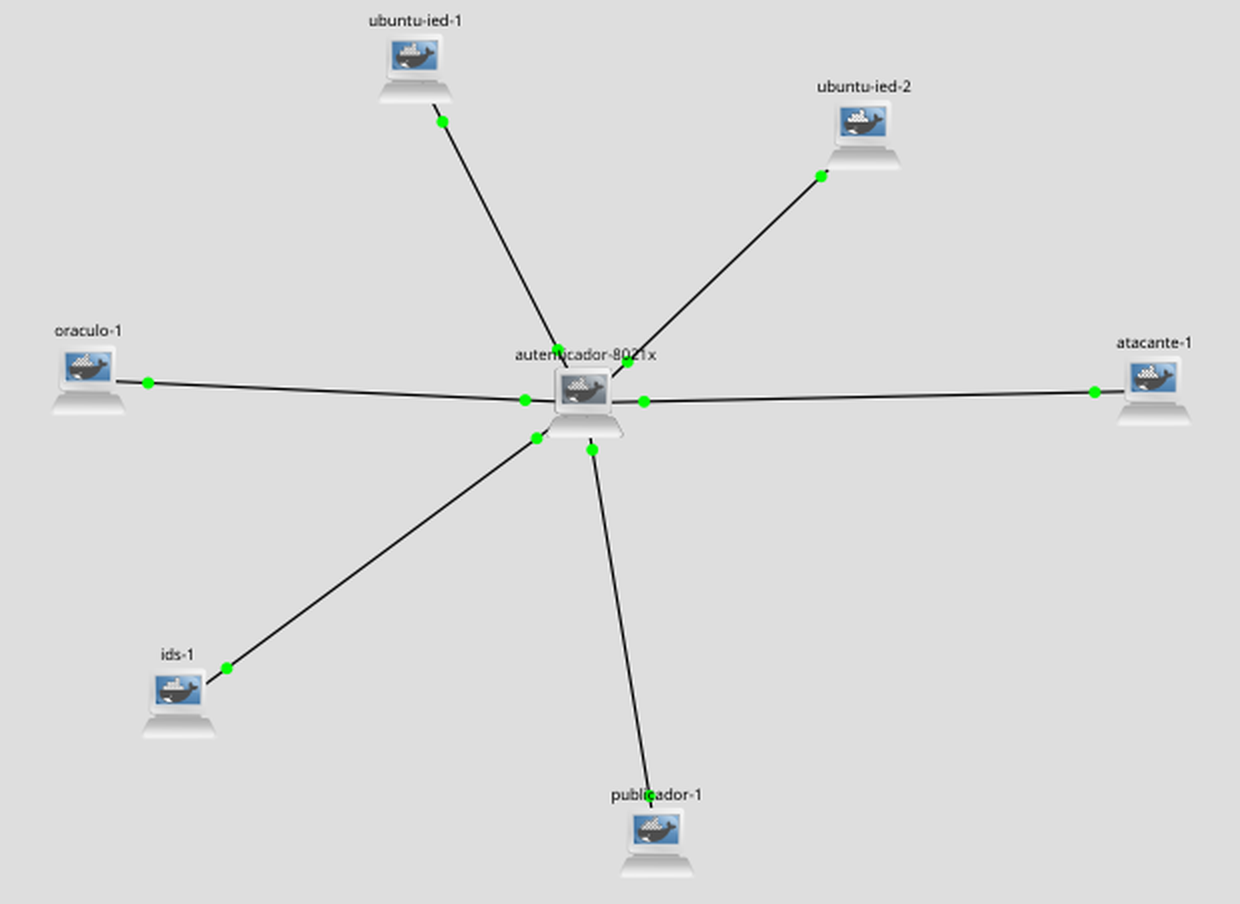
\includegraphics[width=0.8\linewidth]{figuras/gns3_topologia_8021x.png}
\caption{Topologia \texttt{subestacao\_\allowbreak{}8021x} no GNS3 2.2.61 durante a validação de 20/11/2026: sete nós Docker, cada um ligado a uma porta do \texttt{autenticador{-}8021x}, sem \emph{switches} nativos.}\label{fig:3}
\end{figure}

\subsection{Quadro-molde e codec GOOSE}\label{sec:4.2}

Todos os quadros GOOSE do trabalho derivam de um único quadro, capturado de um relé SEL-351, conforme a documentação do projeto. A Tabela~\ref{tab:9} resume seus campos. O codec interpreta o cabeçalho e os campos escalares do PDU e trata o \texttt{allData} como um bloco de bytes opaco, reaproveitado da captura; o valor booleano de estado é localizado pela assinatura TLV de um booleano MMS (\texttt{0x83 0x01 <v>}). A reconstrução do quadro pelo codec é idêntica, byte a byte, ao original, o que é verificado por teste automatizado. Como todos os quadros derivam do molde, a variedade do tráfego é sintética: os ataques alteram, no máximo, \texttt{stNum}, \texttt{sqNum}, \texttt{t}, o MAC de origem, o valor booleano de estado e, nos modos com HMAC, a tag de autenticação (ausente, se o atacante não tem a chave, ou calculada com a chave-mestra, se a tem).

\begin{table}[!t]
\centering
\caption{Campos do quadro-molde.}\label{tab:9}
\footnotesize
\begin{tabularx}{\linewidth}{>{\hsize=0.828\hsize\raggedright\arraybackslash}X>{\hsize=1.172\hsize\raggedright\arraybackslash}X}
\toprule
\textbf{Campo} & \textbf{Valor} \\
\midrule
Tamanho do quadro & 367 bytes \\
MAC de origem / destino & \texttt{00:30:a7:01:b3:16} / \texttt{01:0c:cd:01:00:03} \\
APPID; marcação VLAN & \texttt{0x0003}; ausente \\
\texttt{gocbRef} & \texttt{SEL\_\allowbreak{}351\_\allowbreak{}1CFG/\allowbreak{}LLN0\$\allowbreak{}GO\$\allowbreak{}NewGOOSEMessage} \\
\texttt{datSet}; \texttt{goID} & \texttt{SEL\_\allowbreak{}351\_\allowbreak{}1CFG/\allowbreak{}LLN0\$\allowbreak{}three51to2411}; \texttt{SEL\_\allowbreak{}351\_\allowbreak{}1} \\
\texttt{stNum} / \texttt{sqNum} & 23 / 521 \\
\texttt{timeAllowedToLive}; \texttt{confRev} & 2000; 1 \\
\texttt{allData} & 223 bytes (bloco opaco) \\
\bottomrule
\end{tabularx}
\end{table}

\subsection{Ambientes de avaliação}\label{sec:4.3}

A avaliação usa três ambientes, descritos a seguir; a Tabela~\ref{tab:7} resume seus cenários. Cada um produz evidências de natureza diferente, e seus resultados não são somados.

\emph{4.3.1. Campanha offline.} A campanha constrói os quadros a partir do molde, relê-os com o codec e os entrega diretamente ao monitor do IDS, com um relógio virtual: não há rede, \emph{switch} nem IED. Cada repetição usa um monitor novo, cinco \emph{heartbeats} legítimos de aquecimento a 1 Hz e, depois, apenas o tráfego do atacante; os intervalos entre quadros variam \ensuremath{\pm}10\%, e a semente é fixa (61850). Os cenários são T0 (tráfego legítimo, 60 s, com \emph{heartbeat} a 1 Hz e duas rajadas de 5 pacotes/s), A (flooding, 3 s), B (replay), C1 e C2 (masquerade) e D (suppression), nos modos sem HMAC, com HMAC e com chave comprometida (Seção~\ref{sec:3.4}). São 100 repetições por cenário e modo, e não por parâmetro. No flooding, as 100 repetições percorrem ciclicamente as taxas de 50, 100, 250, 500, 1000 e 2000 pacotes/s, e, no suppression, os saltos de 60, 100, 250, 500, 1000 e 5000; isso dá 17 repetições para cada um dos quatro primeiros valores e 16 para cada um dos dois últimos. No replay, o atraso é sorteado a cada repetição, de forma uniforme, entre 0,5 e 10 s. Em T0, C1 e C2 não há parâmetro. O denominador de cada TPR e do FPR é, portanto, 100 por cenário e modo, agregando os parâmetros do cenário. A sensibilidade do limiar de flooding é varrida à parte (Seção~\ref{sec:6}), para limiares de 10, 20, 40 e 80 pacotes/s, com 100 repetições por combinação de limiar e taxa. \textbf{A campanha é uma reconstrução:} o script de uma campanha anterior do projeto, apresentada no 4.\textordmasculine{} Marco, não foi preservado. Os parâmetros dos cenários seguem os dessa campanha; os detalhes não documentados (duração do flooding, aquecimento, forma das rajadas do tráfego legítimo e método de cronometragem) foram escolhidos na reconstrução. Ela foi executada em Python 3.12.11, em Linux (\emph{kernel} 7.3.4, CachyOS), e durou 70,1 s.

\emph{4.3.2. GNS3 com 802.1X.} A avaliação usa a topologia \texttt{subestacao\_\allowbreak{}8021x} (Figura~\ref{fig:3}), aberta no GNS3 2.2.61 em 20/11/2026: sete nós Docker, a partir de cinco imagens, cada um ligado a uma porta do autenticador, com a PKI de laboratório instalada nos volumes dos nós. Os cenários E0 a E5 (Tabela~\ref{tab:4}) foram executados \textbf{uma vez cada}, seguindo um roteiro, e o \texttt{atacante{-}1} envia o masquerade com o MAC e a credencial de cada cenário. O IDS esteve ativo em E0, E1, E4 e E5: sem verificação de HMAC em E0, E1 e E4 e com verificação (\texttt{{-}{-}auth}) em E5, com uma chave de teste; nesses cenários, o \texttt{publicador{-}1} emite quadros legítimos que estabelecem a referência do \texttt{gocbRef} no IDS (assinados em E5). Em E2, E3 e E4b, o IDS não estava em execução (o roteiro não o inicia em E2 e E3, e no E4b ele havia sido parado), e a evidência de cada um desses cenários é: em E2, o evento \texttt{auth\_\allowbreak{}rejeitada} por certificado revogado, a mensagem do \emph{supplicant} e o \texttt{ping}; em E3, o evento \texttt{auth\_\allowbreak{}rejeitada} por \texttt{mac\_\allowbreak{}divergente}, o conjunto de pares autorizados e o \texttt{ping}; e, em E4b, o contador do \texttt{nftables}. As evidências do conjunto são o log JSONL do autenticador, copiado do volume do nó; os alertas do IDS e o \texttt{tcpdump}, extraídos do contêiner; e saídas de console coladas pelo operador (\texttt{ping} e \texttt{nft list set}). Uma medição auxiliar, feita em ambiente de depuração (contêiner privilegiado, fora do GNS3), registrou o TLS 1.2 como versão negociada (Seção~\ref{sec:2.2}); ela não é um ambiente de avaliação.

\emph{4.3.3. Network namespaces.} O teste roda em um contêiner Docker privilegiado, com o \texttt{hostapd}, o \texttt{wpa\_\allowbreak{}supplicant} (versão 2.10) e o \texttt{nftables} reais; nove clientes, em \emph{namespaces} distintos, são ligados por pares veth à ponte do contêiner, sem passar pela ponte do \emph{host}, que descartaria o EAPOL. A PKI é temporária. O teste não envia tráfego GOOSE: verifica, por \texttt{ping} e pelos eventos do autenticador, quem é autenticado, quem alcança quem e quais motivos de rejeição são registrados. Cada execução faz 30 verificações. Há 11 execuções registradas, todas em 20/11/2026: oito com 30 verificações aprovadas e nenhuma falha; duas com 29 aprovadas e nenhuma falha, de uma versão da suíte com uma verificação a menos; e \textbf{uma com 28 aprovadas e 2 falhas}, a sexta em ordem cronológica. As falhas foram \textquotedblleft{}c1 reautentica sozinho e volta a alcançar c2\textquotedblright{} e \textquotedblleft{}c1 (não revogado) segue alcançando c6\textquotedblright{}, esta dependente da anterior. A causa não está registrada no repositório, e as cinco execuções seguintes registraram 30 verificações aprovadas. A suíte passou de 29 para 30 verificações entre as primeiras execuções, e o README do autenticador registra correções de código nos componentes testados; esses fatos não são relacionados aqui à execução com 28/2. \textbf{As 11 execuções não são amostras independentes}, porque a suíte e o código mudaram durante a série; por isso não calculamos taxas nem intervalos de confiança. Um teste à parte confirma que o \emph{supplicant} embutido nas quatro imagens de nós autentica contra o autenticador (16 verificações, nenhuma falha).

\subsection{Métricas e critérios}\label{sec:4.4}

\emph{Detecção.} \textquotedblleft{}Detectado\textquotedblright{} significa que algum quadro do atacante gerou ao menos um alerta; em T0, qualquer alerta é um falso positivo. Reportamos a taxa de detecção (TPR) por cenário e modo, a taxa de falsos positivos (FPR) em T0 e o intervalo de confiança de 95\% de Wilson. Como o conteúdo dos quadros é determinístico para cada par (modo, parâmetro), e as repetições de um cenário variam apenas no parâmetro (ciclado ou sorteado, Seção~4.3.1) e no tempo (\ensuremath{\pm}10\% nos intervalos), as taxas saem em 0\% ou 100\%, e o intervalo de Wilson (N = 100 por cenário e modo) é o que quantifica a incerteza, e não um desvio entre repetições independentes.

\emph{Latência.} A latência é medida por quadro, com \texttt{perf\_\allowbreak{}counter\_\allowbreak{}ns}, descontando a mediana do custo de uma leitura do cronômetro (cerca de 2 \textmu{}s neste ambiente). Separamos o \emph{parse}, a verificação do HMAC e o processamento no monitor do IDS, e um microbenchmark isolado mede a assinatura e a verificação (20.000 chamadas cada). Como a implementação é em Python, o valor absoluto e o desvio variam entre execuções; interpretamos a ordem de grandeza e as diferenças relativas. Adotamos 4 ms (4.000 \textmu{}s) como critério experimental de viabilidade, uma escolha deste trabalho (Seção~\ref{sec:2.1}), e não como requisito normativo.

\emph{GNS3 e network namespaces.} As evidências desses ambientes são qualitativas ou de contagem: eventos do autenticador, contadores do \texttt{nftables}, alertas do IDS, \texttt{ping} de poucos pacotes e verificações aprovadas ou não. Não calculamos taxas nem intervalos de confiança com elas. Não medimos a latência nem a sobrecarga de autenticação do EAP-TLS em nenhum ambiente.

\subsection{Reprodutibilidade e disponibilidade}\label{sec:4.5}

O código, os scripts da campanha, as evidências dos três ambientes e a medição auxiliar de TLS estão no repositório do projeto (\url{https://github.com/xymotaa/iec61850-security-testbed}), no commit \texttt{e813f70} (o último a alterar o código e as evidências; os posteriores só alteram o artigo). As evidências estão em \texttt{benchmark/\allowbreak{}resultados/\allowbreak{}} (campanha \emph{offline}), \texttt{autenticador{-}8021x/\allowbreak{}evidencias/\allowbreak{}gns3/\allowbreak{}} (GNS3), \texttt{autenticador{-}8021x/\allowbreak{}evidencias/\allowbreak{}} (logs \texttt{teste\_\allowbreak{}netns{-}*.\allowbreak{}log} dos \emph{network namespaces}) e \texttt{autenticador{-}8021x/\allowbreak{}evidencias/\allowbreak{}tls/\allowbreak{}} (medição de TLS). A PKI é de laboratório: as chaves privadas não são versionadas e são geradas por um script do projeto. A campanha \emph{offline} usa semente fixa, e os comandos de cada ambiente estão nos arquivos de documentação do repositório.

\section{Técnicas de defesa e modificações no testbed}\label{sec:5}

Esta seção descreve as três técnicas avaliadas e as alterações feitas no testbed para implementá-las. O modelo de ameaças está na Seção~\ref{sec:3} e os resultados na Seção~\ref{sec:6}; aqui interessam apenas os mecanismos necessários para interpretá-los. Os mecanismos de defesa são ativados conforme a variante experimental utilizada (Seção~\ref{sec:5.4}).

\subsection{IDS de estado}\label{sec:5.1}

O IDS observa passivamente o tráfego GOOSE e mantém, para cada \texttt{gocbRef}, o último \texttt{stNum}, o último \texttt{sqNum} e o último MAC de origem visto. Ele não atua sobre a rede: gera alertas, escritos na saída padrão e, opcionalmente, em um arquivo JSONL. O primeiro quadro de um \texttt{gocbRef} apenas cria a referência e não gera alerta, de modo que o IDS não distingue um publicador legítimo de um falso se o primeiro quadro observado já for forjado.

A Figura~\ref{fig:4} mostra o fluxo de decisão para cada quadro, e a Tabela~\ref{tab:10} resume as regras. A taxa de quadros é verificada primeiro, em uma janela deslizante de 2 s: há alerta quando a taxa média na janela excede 20 pacotes/s, isto é, mais de 40 quadros em 2 s. O alerta é emitido apenas nas bordas, \texttt{flood\_\allowbreak{}start} no início e \texttt{flood\_\allowbreak{}end} no fim, e não a cada quadro. Como o fim de uma rajada não tem um quadro seguinte que o revele, um relógio de reavaliação (\texttt{tick}), chamado cerca de uma vez por segundo, também encerra o estado de flooding. Em seguida, se a autenticação estiver ativa e a verificação falhar, o IDS emite \texttt{auth\_\allowbreak{}fail} e descarta o quadro sem atualizar o estado. Do contrário, aplica as regras de masquerade (MAC diferente do último MAC do \texttt{gocbRef}), replay (par \texttt{(stNum, sqNum)} menor ou igual ao último) e suppression (salto de \texttt{stNum} maior que 50). Um quadro classificado como replay não faz o estado avançar, mas o MAC de origem é atualizado.

\begin{figure}[!t]
\centering
\begin{tikzpicture}[x=1cm,y=1cm,
  dec/.style={caixa, cinza, text width=6.6cm}]
  \node[caixa, text width=6.6cm] (q) at (0,0) {Quadro GOOSE recebido};
  \node[caixa, text width=6.6cm] (taxa) at (0,-1.5) {Taxa de quadros na janela de 2~s acima do limiar (20 pacotes/s)?};
  \node[dec] (aut) at (0,-3.2) {Autenticação ativa e tag HMAC ausente ou inválida?};
  \node[dec] (ref) at (0,-4.8) {Há referência para o \texttt{gocbRef}?};
  \node[caixa, text width=6.6cm] (reg) at (0,-7.0) {Regras de estado\\masquerade: MAC diferente do último visto\\replay: \texttt{(stNum, sqNum)} $\leq$ último par\\suppression: salto de \texttt{stNum} $>$ 50};
  \node[caixa, text width=6.6cm] (upd) at (0,-9.2) {Atualiza o estado: MAC sempre; \texttt{stNum} e \texttt{sqNum} só se não houve replay};
  \node[caixa, text width=4.6cm] (fl) at (9.0,-1.5) {Alerta \texttt{flood\_start} ou \texttt{flood\_end} (só nas bordas); o quadro segue};
  \node[caixa, text width=4.6cm] (af) at (9.0,-3.2) {Alerta \texttt{auth\_fail}; o quadro é descartado e o estado não muda};
  \node[caixa, text width=4.6cm] (cr) at (9.0,-4.8) {Cria a referência (sem alerta) e atualiza o estado};
  \draw[seta] (q) -- (taxa);
  \draw[seta] (taxa) -- (aut);
  \draw[seta] (aut) -- node[right, font=\footnotesize] {não} (ref);
  \draw[seta] (ref) -- node[right, font=\footnotesize] {sim} (reg);
  \draw[seta] (reg) -- (upd);
  \draw[seta, dashed] (taxa) -- node[above, font=\footnotesize] {sim} (fl);
  \draw[seta] (aut) -- node[above, font=\footnotesize] {sim} (af);
  \draw[seta] (ref) -- node[above, font=\footnotesize] {não} (cr);
\end{tikzpicture}

\caption{Fluxo de decisão do monitor de estado do IDS para cada quadro GOOSE recebido.}\label{fig:4}
\end{figure}

\begin{table}[!t]
\centering
\caption{Regras do IDS de estado.}\label{tab:10}
\footnotesize
\begin{tabularx}{\linewidth}{>{\hsize=0.700\hsize\raggedright\arraybackslash}X>{\hsize=2.027\hsize\raggedright\arraybackslash}X>{\hsize=0.532\hsize\raggedright\arraybackslash}X>{\hsize=0.741\hsize\raggedright\arraybackslash}X}
\toprule
\textbf{Regra} & \textbf{Condição de alerta} & \textbf{Parâmetro (padrão)} & \textbf{Alerta} \\
\midrule
Flooding & Taxa média na janela > limiar & Janela de 2 s; 20 pacotes/s & \texttt{flood\_\allowbreak{}start}, \texttt{flood\_\allowbreak{}end} \\
Autenticação (opcional) & Tag HMAC ausente, malformada ou inválida & — & \texttt{auth\_\allowbreak{}fail} \\
Masquerade & MAC de origem \ensuremath{\neq} último MAC do \texttt{gocbRef} & — & \texttt{masquerade} \\
Replay & (\texttt{stNum}, \texttt{sqNum}) \ensuremath{\leq} último par visto & — & \texttt{replay} \\
Suppression & \texttt{stNum} \ensuremath{-} último \texttt{stNum} > limiar & 50 & \texttt{suppression} \\
\bottomrule
\end{tabularx}
\end{table}

Os limiares de flooding e de suppression são escolhas deste trabalho e podem ser alterados por linha de comando (\texttt{{-}{-}flood{-}pps}, \texttt{{-}{-}suppression{-}jump}); a sensibilidade do limiar de flooding é avaliada na Seção~\ref{sec:6}. A regra de masquerade compara apenas o MAC de origem com o do quadro anterior, de modo que um atacante que use o MAC do publicador não a aciona; esse caso é tratado pelas outras camadas.

\subsection{Autenticação por mensagem (HMAC) simulada}\label{sec:5.2}

Para avaliar o efeito de um código de autenticação sobre o IDS, implementamos uma simulação de autenticação por mensagem. Ela é inspirada no princípio da IEC 62351-6 \cit{IEC 2020}{iec62351-6}, que acrescenta um código de autenticação ao GOOSE, mas \textbf{não implementa o perfil da norma} nem é interoperável com ele: o formato do quadro e a gestão de chaves são escolhas deste trabalho, e a única relação com a norma que afirmamos é a do princípio, conforme descrito na literatura \cit{Herath et al. 2025}{herath2025evaluation}.

Cada quadro leva uma tag HMAC-SHA256 de 32 bytes, sem truncamento, calculada com uma chave específica do \texttt{gocbRef}, derivada da chave-mestra por HMAC-SHA256 do texto \texttt{gocbRef:} seguido do próprio \texttt{gocbRef}. A tag cobre os campos \texttt{gocbRef}, \texttt{stNum}, \texttt{sqNum}, \texttt{t} e \texttt{allData}, cada um precedido de seu tamanho em 4 bytes; os campos de \texttt{stNum} e \texttt{sqNum} entram com 8 bytes. A Tabela~\ref{tab:11} lista o que a tag cobre e o que fica de fora. Como a tag não cobre o MAC de origem, o \texttt{timeAllowedToLive}, o \texttt{datSet}, o \texttt{goID}, o \texttt{test}, o \texttt{confRev}, o \texttt{ndsCom}, o \texttt{numDatSetEntries}, o APPID nem a marcação VLAN, o HMAC não protege esses campos contra alteração. A verificação usa \texttt{hmac.\allowbreak{}compare\_\allowbreak{}digest}, e um quadro sem tag ou com tag malformada é tratado como inválido.

A tag é transportada em um trailer TLV após o APDU GOOSE: o byte \texttt{0xA0}, o comprimento em BER e os 32 bytes da tag (Figura~\ref{fig:5}). O comprimento do cabeçalho GOOSE passa a incluir o trailer, e o campo \texttt{Reserved1} carrega o tamanho do trailer, valendo 0 quando não há tag; assim, os quadros sem tag permanecem idênticos, byte a byte, aos do codec original. O uso de \texttt{0xA0} e de \texttt{Reserved1} para essa finalidade é uma escolha do trabalho. O IDS só verifica a tag quando iniciado com \texttt{{-}{-}auth}, e o resultado da verificação entra na decisão descrita na Seção~\ref{sec:5.1}.

\begin{figure}[!t]
\centering
\begin{tikzpicture}[x=1cm,y=1cm,
  cob/.style={caixa, fill=gray!35, minimum height=0.9cm, text width=1.95cm, font=\scriptsize},
  ncob/.style={caixa, minimum height=0.9cm, text width=1.95cm, font=\scriptsize}]
  % linha 1: estrutura do quadro (fora de escala)
  \node[caixa, text width=3.3cm, minimum height=1.3cm, font=\scriptsize] (eth) at (1.9,0) {Cabeçalho Ethernet\\MAC de destino, MAC de origem, VLAN (se houver), EtherType \texttt{0x88B8}};
  \node[caixa, text width=3.9cm, minimum height=1.3cm, font=\scriptsize] (hdr) at (6.35,0) {Cabeçalho GOOSE\\APPID, comprimento (inclui o trailer), \texttt{Reserved1} = tamanho do trailer, \texttt{Reserved2}};
  \node[caixa, text width=2.2cm, minimum height=1.3cm, font=\scriptsize] (apdu) at (9.9,0) {APDU GOOSE\\(campos abaixo)};
  \node[caixa, fill=gray!35, text width=3.0cm, minimum height=1.3cm, font=\scriptsize] (trl) at (13.0,0) {Trailer de autenticação\\\texttt{0xA0}, comprimento (BER), tag HMAC-SHA256 de 32 bytes};
  \draw[seta] (eth) -- (hdr);
  \draw[seta] (hdr) -- (apdu);
  \draw[seta] (apdu) -- (trl);
  % linha 2: campos do APDU
  \node[font=\footnotesize, anchor=west] at (-0.4,-1.7) {Campos do APDU, na ordem do quadro:};
  \node[cob]  (a1) at (1.1,-2.7) {\texttt{gocbRef}};
  \node[ncob] (a2) at (3.3,-2.7) {\texttt{timeAllowed\-ToLive}};
  \node[ncob] (a3) at (5.5,-2.7) {\texttt{datSet}};
  \node[ncob] (a4) at (7.7,-2.7) {\texttt{goID}};
  \node[cob]  (a5) at (9.9,-2.7) {\texttt{t}};
  \node[cob]  (a6) at (12.1,-2.7) {\texttt{stNum}};
  \node[cob]  (b1) at (1.1,-3.9) {\texttt{sqNum}};
  \node[ncob] (b2) at (3.3,-3.9) {\texttt{test}};
  \node[ncob] (b3) at (5.5,-3.9) {\texttt{confRev}};
  \node[ncob] (b4) at (7.7,-3.9) {\texttt{ndsCom}};
  \node[ncob] (b5) at (9.9,-3.9) {\texttt{numDat\-SetEntries}};
  \node[cob]  (b6) at (12.1,-3.9) {\texttt{allData}};
  % legenda
  \node[cob, text width=1.2cm, minimum height=0.5cm] at (1.0,-5.2) {};
  \node[font=\footnotesize, anchor=west] at (1.7,-5.2) {coberto pela tag};
  \node[ncob, text width=1.2cm, minimum height=0.5cm] at (6.0,-5.2) {};
  \node[font=\footnotesize, anchor=west] at (6.7,-5.2) {não coberto};
\end{tikzpicture}

\caption{Quadro GOOSE com o trailer de autenticação: cabeçalho Ethernet, cabeçalho GOOSE (com \texttt{Reserved1} igual ao tamanho do trailer), APDU e trailer (\texttt{0xA0}, comprimento BER, tag de 32 B).}\label{fig:5}
\end{figure}

\begin{table}[!t]
\centering
\caption{Campos do quadro GOOSE cobertos e não cobertos pela tag HMAC.}\label{tab:11}
\footnotesize
\begin{tabularx}{\linewidth}{>{\hsize=0.815\hsize\raggedright\arraybackslash}X>{\hsize=1.185\hsize\raggedright\arraybackslash}X}
\toprule
\textbf{Cobertos} & \textbf{Não cobertos} \\
\midrule
\texttt{gocbRef}, \texttt{stNum}, \texttt{sqNum}, \texttt{t}, \texttt{allData} & \texttt{timeAllowedToLive}, \texttt{datSet}, \texttt{goID}, \texttt{test}, \texttt{confRev}, \texttt{ndsCom}, \texttt{numDatSetEntries}; MAC de origem e de destino; APPID; marcação VLAN \\
\bottomrule
\end{tabularx}
\end{table}

A chave-mestra vem da variável de ambiente \texttt{GOOSE\_\allowbreak{}HMAC\_\allowbreak{}KEY}; se ela não for definida, o IDS usa uma constante pública de teste, \texttt{TEST\_\allowbreak{}MASTER\_\allowbreak{}KEY}, que é também a chave da campanha \emph{offline}. Nos cenários do GNS3 com HMAC (E5), usamos outra chave de teste, \texttt{chave{-}de{-}teste}, passada por \texttt{GOOSE\_\allowbreak{}HMAC\_\allowbreak{}KEY}. \textbf{As duas chaves são públicas e exclusivas do experimento; não protegem nada.} A simulação não tem distribuição nem rotação de chaves. A autenticação HMAC, isoladamente, não impede o replay de um quadro legítimo assinado: uma cópia integral preserva a tag válida. A identificação de duplicatas depende de um mecanismo adicional de controle de estado, como a regra de replay do IDS. No lado do atacante, a opção \texttt{{-}{-}leaked{-}key{-}env} indica uma variável de ambiente com a chave-mestra, usada para assinar os quadros de flooding, masquerade e suppression; sem ela, os quadros saem sem tag, e o replay, que reenvia um quadro já assinado, não é afetado. \textquotedblleft{}Chave vazada\textquotedblright{} refere-se, portanto, à chave-mestra inteira, uma hipótese mais forte do que o vazamento da chave de um único fluxo.

\subsection{Controle de acesso 802.1X com EAP-TLS}\label{sec:5.3}

O controle de acesso usa o padrão IEEE 802.1X \cit{IEEE 2020}{ieee8021x} com EAP-TLS \cit{Simon et al. 2008}{rfc5216}, implementado com componentes reais: o \texttt{hostapd}, o \texttt{wpa\_\allowbreak{}supplicant} e o \texttt{nftables}. A Figura~\ref{fig:6} mostra a arquitetura e o fluxo de decisão.

\textbf{Arquitetura.} O \texttt{autenticador{-}8021x} é um único contêiner que forma uma ponte de camada 2 (\texttt{br0}), com 9 portas por padrão, à qual cada nó se liga. O \texttt{hostapd} roda com o driver \emph{wired}, em um processo, com um arquivo de configuração por porta. O servidor de autenticação EAP está embutido no \texttt{hostapd}, sem servidor RADIUS externo, e aceita qualquer identidade (\texttt{eap\_\allowbreak{}user: * TLS}), de modo que a decisão fica a cargo da verificação do certificado e do inventário. A reautenticação ocorre a cada 600 s. Os nós usam um \emph{supplicant} opcional (\texttt{AUTH\_\allowbreak{}8021X=1}), com \texttt{wpa\_\allowbreak{}supplicant} em modo \emph{wired}, \texttt{eap=TLS} e verificação do sufixo de domínio do servidor; um \emph{watchdog} o reinicia após uma perda de portadora ou após 20 s sem autorização.

\textbf{PKI.} Uma PKI de laboratório, gerada por script, emite uma CA (válida por 3650 dias), um certificado de servidor com \texttt{serverAuth} e certificados de cliente com \texttt{clientAuth} por nó (825 dias), todos com RSA de 2048 bits e SHA-256, mais uma lista de revogação (CRL). O \texttt{hostapd} recebe a CA e a CRL concatenadas, com \texttt{check\_\allowbreak{}crl=1} e recarga da CRL a cada 60 s. As chaves privadas não são versionadas.

\textbf{Decisão de acesso.} A autenticação do certificado não basta para liberar o tráfego: um supervisor lê o log do \texttt{hostapd} (a interface de controle expõe apenas a identidade declarada pelo cliente) e cruza o nome comum (CN) do certificado com um inventário que associa cada CN ao MAC autorizado, gerado a partir do SCD. A autorização só é concedida se o certificado for aceito \textbf{e} o MAC de origem da porta coincidir com o MAC do inventário para aquele CN. O resultado alimenta o \texttt{nftables}, que opera no gancho \emph{forward} da ponte, com política de descarte: um quadro é encaminhado se vier de uma porta confiável ou se o par (interface de entrada, MAC de origem) estiver no conjunto de pares autorizados e a porta de saída tiver ao menos um dispositivo autorizado. O EAPOL (01:80:C2:00:00:03) não passa por essas regras, pois é tratado pelo autenticador. As regras são carregadas antes de as portas entrarem na ponte, de modo que o sistema falha fechado. Os quadros descartados são contados em um conjunto dinâmico, com validade de 120 s, e geram eventos periódicos. A lista de portas confiáveis existe como mecanismo de exceção, mas fica vazia e não foi usada em nenhum cenário.

O supervisor escreve eventos JSONL: \texttt{auth\_\allowbreak{}aceita}, \texttt{auth\_\allowbreak{}rejeitada}, \texttt{sessao\_\allowbreak{}encerrada} e \texttt{quadro\_\allowbreak{}descartado}. A Tabela~\ref{tab:12} lista os motivos de rejeição.

\begin{figure}[!t]
\centering
\begin{minipage}[t]{0.49\linewidth}
\centering
\begin{tikzpicture}[x=1cm,y=1cm, every node/.style={font=\scriptsize},
  no/.style={caixa, font=\scriptsize, text width=2.2cm, inner sep=2pt}]
  \node[no] (n0) at (0,0)    {\texttt{ubuntu-ied-1}};
  \node[no] (n1) at (0,-0.98){\texttt{ubuntu-ied-2}};
  \node[no] (n2) at (0,-1.96) {\texttt{oraculo-1}};
  \node[no] (n3) at (0,-2.94){\texttt{ids-1}};
  \node[no] (n4) at (0,-3.92) {\texttt{publicador-1}};
  \node[no] (n5) at (0,-4.9){\texttt{atacante-1}};
  \node[draw, rounded corners=3pt, minimum width=3.4cm, minimum height=5.7cm, fill=gray!8, anchor=north west] (aut) at (2.0,0.5) {};
  \node[font=\scriptsize\bfseries, anchor=north] at (3.7,0.4) {\texttt{autenticador-8021x}};
  \node[caixa, font=\scriptsize, text width=3.0cm] at (3.7,-1.15) {\texttt{hostapd}, um processo por porta (EAP-TLS)};
  \node[caixa, font=\scriptsize, text width=3.0cm] at (3.7,-2.6) {Supervisor: lê o log do \texttt{hostapd} e consulta o inventário CN$\rightarrow$MAC};
  \node[caixa, font=\scriptsize, text width=3.0cm] at (3.7,-4.1) {\texttt{nftables}: ponte \texttt{br0}, gancho \emph{forward}, política de descarte};
  \foreach \i in {0,1,2,3,4,5}{
    \draw (n\i.east) -- node[above, font=\tiny, pos=0.5] {eth\i} (2.0,-0.98*\i);
  }
\end{tikzpicture}

\footnotesize (a)
\end{minipage}%
\hfill
\begin{minipage}[t]{0.49\linewidth}
\centering
\begin{tikzpicture}[x=1cm,y=1cm, every node/.style={font=\scriptsize},
  d/.style={caixa, cinza, font=\scriptsize, text width=2.7cm, inner sep=2pt},
  r/.style={caixa, font=\scriptsize, text width=2.5cm, inner sep=2pt}]
  \node[caixa, font=\scriptsize, text width=2.7cm, inner sep=2pt] (e) at (0,0) {Handshake EAP-TLS};
  \node[d] (c) at (0,-1.3) {Certificado e CRL válidos?};
  \node[d] (i) at (0,-2.8) {CN no inventário?};
  \node[d] (m) at (0,-4.1) {MAC da porta é um dos MACs do CN?};
  \node[caixa, font=\scriptsize, text width=2.7cm, inner sep=2pt] (ok) at (0,-5.4) {Par (porta, MAC) autorizado no \texttt{nftables}};
  \node[r] (r1) at (3.7,-1.3) {\texttt{sem\_\allowbreak certificado}, \texttt{certificado\_\allowbreak invalido}, \texttt{certificado\_\allowbreak revogado} ou \texttt{falha\_\allowbreak eap}};
  \node[r] (r2) at (3.7,-2.8) {\texttt{cn\_\allowbreak fora\_\allowbreak do\_\allowbreak inventario}};
  \node[r] (r3) at (3.7,-4.1) {\texttt{mac\_\allowbreak divergente}};
  \draw[seta] (e) -- (c);
  \draw[seta] (c) -- node[left, font=\tiny] {sim} (i);
  \draw[seta] (i) -- node[left, font=\tiny] {sim} (m);
  \draw[seta] (m) -- node[left, font=\tiny] {sim} (ok);
  \draw[seta] (c) -- node[above, font=\tiny] {não} (r1);
  \draw[seta] (i) -- node[above, font=\tiny] {não} (r2);
  \draw[seta] (m) -- node[above, font=\tiny] {não} (r3);
\end{tikzpicture}

\footnotesize (b)
\end{minipage}

\caption{(a) Arquitetura do \texttt{autenticador{-}8021x}: nós ligados às portas da ponte \texttt{br0}, um processo \texttt{hostapd} por porta, supervisor com o inventário CN\ensuremath{\rightarrow}MAC e regras \texttt{nftables} no gancho \emph{forward}. (b) Fluxo de decisão: EAP-TLS \ensuremath{\rightarrow} validação do certificado e da CRL \ensuremath{\rightarrow} CN no inventário \ensuremath{\rightarrow} MAC da porta igual ao do inventário \ensuremath{\rightarrow} autorização do par (porta, MAC) no \texttt{nftables}; cada falha gera um evento \texttt{auth\_\allowbreak{}rejeitada} com o motivo correspondente.}\label{fig:6}
\end{figure}

\begin{table}[!t]
\centering
\caption{Motivos de rejeição registrados pelo autenticador.}\label{tab:12}
\footnotesize
\begin{tabularx}{\linewidth}{>{\hsize=0.512\hsize\raggedright\arraybackslash}X>{\hsize=1.488\hsize\raggedright\arraybackslash}X}
\toprule
\textbf{Motivo} & \textbf{Situação} \\
\midrule
\texttt{sem\_\allowbreak{}certificado} & O cliente recusa o EAP-TLS (sem credencial configurada) \\
\texttt{certificado\_\allowbreak{}invalido} & Erro de TLS na verificação do certificado, exceto revogação \\
\texttt{certificado\_\allowbreak{}revogado} & Erro de TLS indicando revogação (código X509 23, da CRL) \\
\texttt{cn\_\allowbreak{}fora\_\allowbreak{}do\_\allowbreak{}inventario} & CN do certificado ausente do inventário \\
\texttt{mac\_\allowbreak{}divergente} & CN presente no inventário, mas MAC de origem fora do conjunto de MACs autorizados para esse CN \\
\texttt{falha\_\allowbreak{}eap} & EAP termina em falha sem erro de certificado \\
\bottomrule
\end{tabularx}
\end{table}

Quanto ao TLS, a configuração do projeto não fixa a versão. Em uma medição de depuração, fora do GNS3 (Seção~4.3.2), o EAP-TLS negociou o TLS 1.2, e por isso a RFC 5216 \cit{Simon et al. 2008}{rfc5216} é a referência aplicável; a RFC 9190 \cit{Preuß Mattsson e Sethi 2022}{rfc9190} só se aplicaria com TLS 1.3. Habilitar o TLS 1.3 nas duas pontas também resultou em TLS 1.2, sem que a causa tenha sido investigada. O vínculo entre certificado e MAC é uma decisão deste trabalho, e não uma exigência do 802.1X.

\subsection{Modificações no testbed}\label{sec:5.4}

As modificações abaixo preservam o comportamento da topologia padrão quando os recursos adicionais não são habilitados. No IDS, a opção \texttt{{-}{-}auth}, o parâmetro \texttt{auth\_\allowbreak{}valid} e o evento \texttt{auth\_\allowbreak{}fail}; sem eles, não há verificação de HMAC. No codec GOOSE, o trailer de autenticação (tag \texttt{0xA0}, \texttt{Reserved1}); sem tag, os quadros são idênticos, byte a byte, aos do codec original. No atacante, a opção \texttt{{-}{-}leaked{-}key{-}env}, que assina os quadros de flooding, masquerade e suppression; sem ela, os quadros de ataque saem sem tag HMAC. Na topologia e na identidade, \texttt{ATACANTE\_\allowbreak{}IP} e o uso da imagem do atacante como \texttt{publicador{-}1}; sem \texttt{ATACANTE\_\allowbreak{}IP}, a imagem usa o IP padrão do atacante (192.168.10.40). Nas imagens dos nós, o \emph{supplicant} 802.1X embutido nas quatro imagens, desligado por padrão (\texttt{AUTH\_\allowbreak{}8021X=1} o ativa). No gerador de topologia, a variante \texttt{{-}{-}8021x}, o inventário nome\ensuremath{\rightarrow}MAC e o MAC fixo por nó; sem a variante, a topologia padrão, com \emph{switches}. Também foram acrescentados, como componentes adicionais usados só na variante \texttt{{-}{-}8021x}, a imagem \texttt{autenticador{-}8021x} (\texttt{hostapd}, supervisor e \texttt{nftables}), o script de PKI e o instalador nos volumes dos nós; e, para a avaliação, a campanha \emph{offline} e a varredura do limiar do IDS.

\section{Resultados e análise}\label{sec:6}

Esta seção apresenta os resultados em três níveis de evidência, que não são somados. Os resultados \textbf{medidos} vêm da campanha \emph{offline} (Seções~\ref{sec:6.1} a \ref{sec:6.3}), com N = 100 por cenário e modo. As evidências \textbf{qualitativas} vêm das execuções no GNS3 (Seção~\ref{sec:6.4}), com uma execução por cenário. As \textbf{limitações} do que foi medido estão na Seção~\ref{sec:6.5} e são discutidas na Seção~\ref{sec:7}. Os cenários seguem a nomenclatura da Seção~\ref{sec:3}: T0 (tráfego legítimo), A (flooding), B (replay), C1 e C2 (masquerade) e D (suppression).

\subsection{Detecção pelo IDS na campanha \emph{offline}}\label{sec:6.1}

A Tabela~\ref{tab:13} mostra as detecções por cenário e modo. Para 0/100, o intervalo de Wilson de 95\% é [0,0\%; 3,7\%], e para 100/100 é [96,3\%; 100,0\%]. Como o conteúdo dos quadros é determinístico para cada par (modo, parâmetro) (Seção~\ref{sec:4.4}), os resultados saem em 0\% ou 100\%, e a tabela indica qual regra cobre qual cenário, não uma estimativa de desempenho em tráfego real.

\begin{table}[!t]
\centering
\caption{Detecções por cenário e modo (N = 100 por célula); entre parênteses, os tipos de alerta observados. No cenário T0, a medida é o falso positivo (FPR).}\label{tab:13}
\footnotesize
\begin{tabularx}{\linewidth}{>{\hsize=1.074\hsize\raggedright\arraybackslash}X>{\hsize=0.900\hsize\raggedright\arraybackslash}X>{\hsize=1.125\hsize\raggedright\arraybackslash}X>{\hsize=0.900\hsize\raggedright\arraybackslash}X}
\toprule
\textbf{Cenário} & \textbf{Sem HMAC} & \textbf{HMAC, atacante sem a chave} & \textbf{HMAC, chave vazada} \\
\midrule
T0 (FPR) & 0/100 & 0/100 & 0/100 \\
A (flooding) & 100/100 (\texttt{flood\_\allowbreak{}start}) & 100/100 (\texttt{auth\_\allowbreak{}fail}, \texttt{flood\_\allowbreak{}start}) & 100/100 (\texttt{flood\_\allowbreak{}start}) \\
B (replay) & 100/100 (\texttt{replay}) & 100/100 (\texttt{replay}) & 100/100 (\texttt{replay}) \\
C1 (masquerade, MAC do publicador) & \textbf{0/100} & 100/100 (\texttt{auth\_\allowbreak{}fail}) & \textbf{0/100} \\
C2 (masquerade, outro MAC) & 100/100 (\texttt{masquerade}) & 100/100 (\texttt{auth\_\allowbreak{}fail}) & 100/100 (\texttt{masquerade}) \\
D (suppression) & 100/100 (\texttt{suppression}) & 100/100 (\texttt{auth\_\allowbreak{}fail}) & 100/100 (\texttt{suppression}) \\
\bottomrule
\end{tabularx}
\end{table}

Os resultados mostram quatro pontos.

\begin{itemize}
\item \textbf{Falsos positivos.} Em T0, nenhum alerta ocorreu nos três modos. Esse resultado vale para o tráfego sintético desta campanha (um \emph{heartbeat} de 1 Hz e rajadas de 5 pacotes/s).
\item \textbf{C1.} O masquerade com o MAC do publicador clonado não é detectado sem HMAC nem com a chave vazada, porque o quadro forjado é consistente com o estado do IDS, que só compara o MAC com o do quadro anterior. Com HMAC e sem a chave, o mesmo ataque é detectado em todas as repetições, pelo alerta \texttt{auth\_\allowbreak{}fail}. A tag, portanto, torna detectável um ataque que o IDS de estado não vê; a chave vazada elimina esse ganho.
\item \textbf{C2.} O IDS de estado detecta o masquerade por \texttt{masquerade} sem HMAC e com a chave vazada. Com HMAC e sem a chave, o alerta registrado é \texttt{auth\_\allowbreak{}fail}, porque o IDS descarta o quadro antes de aplicar a regra de MAC (Seção~\ref{sec:5.1}).
\item \textbf{B.} O replay de um quadro assinado é detectado em todos os modos, e apenas pelo alerta \texttt{replay}: a tag do quadro copiado é válida, e a detecção depende do estado do IDS (Seção~\ref{sec:5.2}).
\end{itemize}

Essas taxas descrevem as regras e os parâmetros desta campanha, e não permitem concluir superioridade sobre outras abordagens, como as que usam aprendizado de máquina.

\subsection{Sensibilidade do limiar de flooding}\label{sec:6.2}

A Figura~\ref{fig:7} mostra como o limiar de flooding afeta a detecção de ataques e os falsos positivos. Cada ponto usa 100 repetições, com limiares de 10, 20, 40 e 80 pacotes/s. O painel (a) varia a taxa do ataque (de 5 a 2000 pacotes/s) e o painel (b) varia a taxa de uma rajada legítima (de 5 a 60 pacotes/s).

\begin{figure}[!t]
\centering
\pgfplotsset{
  sens/.style={width=0.97\linewidth, height=5.2cm, ymin=-0.03, ymax=1.05,
    ytick={0,0.25,0.5,0.75,1}, yticklabels={0\%,25\%,50\%,75\%,100\%},
    grid=major, grid style={gray!25}, tick label style={font=\scriptsize},
    label style={font=\footnotesize}, legend style={font=\scriptsize, draw=gray}}}
\begin{minipage}[t]{0.5\linewidth}
\centering
\begin{tikzpicture}
\begin{axis}[sens, xmode=log, xmin=4, xmax=2500, xlabel={Taxa do ataque (pacotes/s)}, ylabel={Taxa de detecção}, xtick={10,100,1000}, legend columns=4, legend to name=legfig7]
\addplot[mark=square*, solid, color=black, mark size=1.6pt] coordinates {(5,0.0000) (10,0.7200) (15,1.0000) (18,1.0000) (20,1.0000) (22,1.0000) (25,1.0000) (30,1.0000) (35,1.0000) (40,1.0000) (50,1.0000) (60,1.0000) (80,1.0000) (100,1.0000) (250,1.0000) (500,1.0000) (1000,1.0000) (2000,1.0000)};
\addlegendentry{limiar 10}
\addplot[mark=triangle*, dashed, color=gray!70!black, mark size=1.6pt] coordinates {(5,0.0000) (10,0.0000) (15,0.0000) (18,0.0000) (20,0.8200) (22,1.0000) (25,1.0000) (30,1.0000) (35,1.0000) (40,1.0000) (50,1.0000) (60,1.0000) (80,1.0000) (100,1.0000) (250,1.0000) (500,1.0000) (1000,1.0000) (2000,1.0000)};
\addlegendentry{limiar 20}
\addplot[mark=o, dotted, thick, color=black!55, mark size=1.6pt] coordinates {(5,0.0000) (10,0.0000) (15,0.0000) (18,0.0000) (20,0.0000) (22,0.0000) (25,0.0000) (30,0.0000) (35,0.0000) (40,0.8100) (50,1.0000) (60,1.0000) (80,1.0000) (100,1.0000) (250,1.0000) (500,1.0000) (1000,1.0000) (2000,1.0000)};
\addlegendentry{limiar 40}
\addplot[mark=diamond*, dash dot, color=black!85, mark size=1.6pt] coordinates {(5,0.0000) (10,0.0000) (15,0.0000) (18,0.0000) (20,0.0000) (22,0.0000) (25,0.0000) (30,0.0000) (35,0.0000) (40,0.0000) (50,0.0000) (60,0.0000) (80,0.7800) (100,1.0000) (250,1.0000) (500,1.0000) (1000,1.0000) (2000,1.0000)};
\addlegendentry{limiar 80}
\end{axis}
\end{tikzpicture}

\footnotesize (a)
\end{minipage}%
\begin{minipage}[t]{0.5\linewidth}
\centering
\begin{tikzpicture}
\begin{axis}[sens, xmin=3, xmax=62, xtick={10,20,30,40,60}, xlabel={Rajada legítima (pacotes/s)}, ylabel={Taxa de falsos positivos}]
\addplot[mark=square*, solid, color=black, mark size=1.6pt] coordinates {(5,0.0000) (10,0.7700) (15,1.0000) (20,1.0000) (30,1.0000) (40,1.0000) (60,1.0000)};
\addplot[mark=triangle*, dashed, color=gray!70!black, mark size=1.6pt] coordinates {(5,0.0000) (10,0.0000) (15,0.0000) (20,0.7300) (30,1.0000) (40,1.0000) (60,1.0000)};
\addplot[mark=o, dotted, thick, color=black!55, mark size=1.6pt] coordinates {(5,0.0000) (10,0.0000) (15,0.0000) (20,0.0000) (30,0.0000) (40,0.7300) (60,1.0000)};
\addplot[mark=diamond*, dash dot, color=black!85, mark size=1.6pt] coordinates {(5,0.0000) (10,0.0000) (15,0.0000) (20,0.0000) (30,0.0000) (40,0.0000) (60,0.0000)};
\end{axis}
\end{tikzpicture}

\footnotesize (b)
\end{minipage}

\vspace{3pt}
\pgfplotslegendfromname{legfig7}

\caption{Sensibilidade do limiar de flooding do IDS (100 repetições por ponto): (a) taxa de detecção em função da taxa do ataque; (b) taxa de falsos positivos em função da taxa de uma rajada legítima, para os limiares de 10, 20, 40 e 80 pacotes/s.}\label{fig:7}
\end{figure}

Em ambos os painéis, a transição ocorre onde a taxa se iguala ao limiar. Abaixo do limiar, a taxa de detecção e a de falsos positivos são de 0\%. Com a taxa igual ao limiar, ficam entre 72\% e 82\% na detecção (72\%, 82\%, 81\% e 78\% para os limiares 10, 20, 40 e 80) e em 73\% a 77\% nos falsos positivos (77\%, 73\% e 73\% para os limiares 10, 20 e 40). Na primeira taxa amostrada acima do limiar, chegam a 100\%: 15 para o limiar 10, 22 para o 20, 50 para o 40 e 100 para o 80. Esse comportamento é compatível com a regra de alerta, que exige uma taxa estritamente maior que o limiar, combinada com a variação de \ensuremath{\pm}10\% nos intervalos (Seção~4.3.1); não testamos essa explicação isoladamente.

O limiar define, portanto, uma faixa de operação: um ataque mais lento que o limiar não é detectado (por exemplo, com limiar 80, os ataques de 50 e de 60 pacotes/s têm taxa de detecção 0), e uma rajada legítima mais rápida o dispara. O limiar de 20 pacotes/s, usado na campanha, separa as rajadas legítimas testadas de até 15 pacotes/s dos ataques testados a partir de 22 pacotes/s; nada se mediu para rajadas entre 15 e 20 pacotes/s. As rajadas legítimas são hipóteses de teste, e não medidas de uma subestação, e para o limiar 80 a maior rajada testada (60 pacotes/s) é inferior ao limiar, de modo que seu ponto de transição não aparece no painel (b).

\subsection{Latência por quadro}\label{sec:6.3}

A Tabela~\ref{tab:14} resume o tempo gasto por quadro em cada etapa do processamento. Os valores são médias por repetição, e as faixas mostram o menor e o maior valor entre os seis cenários de cada modo; o microbenchmark mede apenas a assinatura e a verificação, com 20.000 chamadas cada.

\begin{table}[!t]
\centering
\caption{Latência por quadro na campanha \emph{offline} (\textmu{}s): faixa entre cenários das médias por repetição e microbenchmark do HMAC.}\label{tab:14}
\footnotesize
\begin{tabularx}{\linewidth}{>{\hsize=1.497\hsize\raggedright\arraybackslash}X>{\hsize=0.950\hsize\raggedright\arraybackslash}X>{\hsize=0.979\hsize\raggedright\arraybackslash}X>{\hsize=0.970\hsize\raggedright\arraybackslash}X>{\hsize=0.605\hsize\raggedright\arraybackslash}X}
\toprule
\textbf{Modo} & \textbf{\emph{Parse}} & \textbf{Verificação do HMAC} & \textbf{Processamento no IDS} & \textbf{Soma das médias} \\
\midrule
Sem HMAC & 29,3 a 61,1 & não se aplica & 5,6 a 11,6 & 36 a 73 \\
HMAC, atacante sem a chave & 32,2 a 50,6 & 2,1 a 15,7 & 4,6 a 17,9 & 50 a 84 \\
HMAC, chave vazada & 39,5 a 57,6 & 13,6 a 21,1 & 6,9 a 16,7 & 60 a 95 \\
\bottomrule
\end{tabularx}
\vspace{6pt}
\footnotesize
\begin{tabularx}{\linewidth}{>{\hsize=2.043\hsize\raggedright\arraybackslash}X>{\hsize=0.662\hsize\raggedright\arraybackslash}X>{\hsize=0.662\hsize\raggedright\arraybackslash}X>{\hsize=0.662\hsize\raggedright\arraybackslash}X>{\hsize=0.970\hsize\raggedright\arraybackslash}X}
\toprule
\textbf{Microbenchmark} & \textbf{Média} & \textbf{Mediana} & \textbf{P99} & \textbf{Desvio-padrão} \\
\midrule
Assinatura (\texttt{sign}) & 12,08 & 11,04 & 26,26 & 18,16 \\
Verificação (\texttt{verify}) & 12,85 & 11,53 & 35,34 & 5,50 \\
\bottomrule
\end{tabularx}
\end{table}

A leitura é a seguinte.

\begin{itemize}
\item \textbf{Verificação.} Uma tag válida custa de 11 a 21 \textmu{}s, em linha com o microbenchmark (12,85 \textmu{}s em média). Uma tag ausente ou inválida custa de 2 a 3 \textmu{}s, porque a verificação termina cedo. Por isso, o custo da verificação só deve ser comparado entre quadros de mesma natureza.
\item \textbf{Peso relativo.} O \emph{parse} do codec é a etapa mais cara em todos os modos, em média mais que a verificação do HMAC.
\item \textbf{Ordem de grandeza.} A maior soma das médias, 95 \textmu{}s (modo com chave vazada, cenário D), corresponde a cerca de 2,4\% do critério experimental de 4 ms (Seção~\ref{sec:4.4}). Esse critério é uma escolha deste trabalho, e a comparação cobre apenas o processamento por quadro em Python.
\end{itemize}

Esses valores não incluem rede, fila nem \emph{hardware} de IED, e variam entre execuções (Seção~\ref{sec:4.4}); interpretamos a ordem de grandeza. \textbf{Não medimos a latência nem a sobrecarga do EAP-TLS em nenhum ambiente, e este trabalho não afirma que ele atenda ao critério de 4 ms.}

\subsection{Camadas combinadas no GNS3}\label{sec:6.4}

A Tabela~\ref{tab:15} resume os cenários executados no GNS3 (Seção~4.3.2), cada um \textbf{uma vez}, em 20/11/2026. Na linha de base, o log do autenticador registra cinco \texttt{auth\_\allowbreak{}aceita} (\texttt{ubuntu{-}ied{-}1}, \texttt{ubuntu{-}ied{-}2}, \texttt{oraculo{-}1}, \texttt{ids{-}1} e \texttt{publicador{-}1}) e nenhuma para o \texttt{atacante{-}1}; o \texttt{ping} de \texttt{ubuntu{-}ied{-}1} para \texttt{ubuntu{-}ied{-}2} retornou 3/3. As evidências são de natureza diferente (log do autenticador, saída de console, contador do \texttt{nftables} e alertas do IDS), e a coluna final identifica a de cada linha. A Figura~\ref{fig:8} mostra, para cada cenário, qual camada atuou e de que forma.

\begin{table}[!t]
\centering
\caption{Cenários E0 a E5 no GNS3 (uma execução por cenário): efeito observado e evidência.}\label{tab:15}
\footnotesize
\begin{tabularx}{\linewidth}{>{\hsize=1.100\hsize\raggedright\arraybackslash}X>{\hsize=1.171\hsize\raggedright\arraybackslash}X>{\hsize=0.729\hsize\raggedright\arraybackslash}X}
\toprule
\textbf{Cenário (credencial; MAC)} & \textbf{Efeito observado} & \textbf{Evidência} \\
\midrule
E0: 802.1X desativado; C1 & \texttt{ping} do atacante 3/3 (RTT médio 0,468 ms); nenhum alerta do IDS registrado & Console; \texttt{alertas\_\allowbreak{}e0.\allowbreak{}jsonl} (vazio) \\
E1: sem credencial; MAC do publicador & \texttt{ping} 0/3 (\emph{Destination Host Unreachable}); \texttt{quadro\_\allowbreak{}descartado} na porta do atacante, com o MAC do publicador (motivo \texttt{origem\_\allowbreak{}nao\_\allowbreak{}autorizada}); nenhum alerta do IDS registrado & Console; log do autenticador; \texttt{alertas\_\allowbreak{}e1.\allowbreak{}jsonl} (vazio) \\
E2: certificado revogado & \texttt{auth\_\allowbreak{}rejeitada} com motivo \texttt{certificado\_\allowbreak{}revogado}; \emph{supplicant}: porta não autorizada após 15 s; \texttt{ping} 0/3 & Log do autenticador; console \\
E3: certificado válido do nó comprometido (CN \texttt{atacante{-}comprometido}, vinculado ao MAC do atacante); MAC de um IED & TLS aceito (o \emph{supplicant} imprime porta autorizada), mas \texttt{auth\_\allowbreak{}rejeitada} com motivo \texttt{mac\_\allowbreak{}divergente}; \texttt{ping} 0/3 & Log do autenticador; console \\
E4: certificado válido; MAC próprio (C2) & Autentica; o quadro forjado chega ao IDS (\texttt{tcpdump}); alerta \texttt{masquerade} & \texttt{tcpdump\_\allowbreak{}e4.\allowbreak{}txt}; \texttt{alertas\_\allowbreak{}e4.\allowbreak{}jsonl} \\
E4b: certificado válido; MAC do publicador & Conjunto \texttt{descartados} do \texttt{nftables}: par (porta do atacante, MAC do publicador), 5 pacotes, 1760 B & Console (\texttt{nft list set}) \\
E5 (i): HMAC; sem a chave; MAC próprio & Alerta \texttt{auth\_\allowbreak{}fail} & \texttt{alertas\_\allowbreak{}e5.\allowbreak{}jsonl} \\
E5 (ii): HMAC; chave vazada; MAC próprio & Alerta \texttt{masquerade} & \texttt{alertas\_\allowbreak{}e5.\allowbreak{}jsonl} \\
E5 (iii): HMAC; chave vazada; MAC do publicador & Nenhum alerta novo registrado; conjunto \texttt{descartados}: mesmo par, 5 pacotes, 1930 B & \texttt{alertas\_\allowbreak{}e5.\allowbreak{}jsonl}; console (\texttt{nft list set}) \\
\bottomrule
\end{tabularx}
\end{table}

\begin{figure}[!t]
\centering
\begin{tikzpicture}[x=1cm,y=1cm,
  c/.style={draw, minimum height=0.72cm, align=center, font=\scriptsize, inner sep=2pt},
  blk/.style={c, fill=gray!50, text width=3.3cm},
  alr/.style={c, fill=gray!20, text width=3.3cm, line width=1.2pt},
  nul/.style={c, text width=3.3cm},
  nex/.style={c, text width=3.3cm, dashed, text=gray!70!black},
  lab/.style={c, text width=1.7cm, font=\scriptsize\bfseries},
  hd/.style={c, minimum height=0.8cm, font=\scriptsize\bfseries, fill=white, text width=3.3cm}]
  \node[hd, text width=1.7cm] at (0,0) {Cenário};
  \node[hd] at (2.75,0) {802.1X (autenticador)};
  \node[hd] at (6.15,0) {HMAC (verificação no IDS)};
  \node[hd] at (9.55,0) {IDS (regras de estado)};
  % linhas (y decrescente)
  \node[lab] at (0,-0.78) {E0};
  \node[nex] at (2.75,-0.78) {desativado};
  \node[nex] at (6.15,-0.78) {inativo};
  \node[nul] at (9.55,-0.78) {sem alerta registrado};
  \node[lab] at (0,-1.5) {E1};
  \node[blk] at (2.75,-1.5) {bloqueio};
  \node[nex] at (6.15,-1.5) {inativo};
  \node[nul] at (9.55,-1.5) {sem alerta registrado};
  \node[lab] at (0,-2.22) {E2};
  \node[blk] at (2.75,-2.22) {bloqueio};
  \node[nex] at (6.15,-2.22) {inativo};
  \node[nex] at (9.55,-2.22) {não em execução};
  \node[lab] at (0,-2.94) {E3};
  \node[blk] at (2.75,-2.94) {bloqueio};
  \node[nex] at (6.15,-2.94) {inativo};
  \node[nex] at (9.55,-2.94) {não em execução};
  \node[lab] at (0,-3.66) {E4};
  \node[nul] at (2.75,-3.66) {sem bloqueio};
  \node[nex] at (6.15,-3.66) {inativo};
  \node[alr] at (9.55,-3.66) {alerta (\texttt{masquerade})};
  \node[lab] at (0,-4.38) {E4b};
  \node[blk] at (2.75,-4.38) {bloqueio};
  \node[nex] at (6.15,-4.38) {inativo};
  \node[nex] at (9.55,-4.38) {não em execução};
  \node[lab] at (0,-5.1) {E5 (i)};
  \node[nul] at (2.75,-5.1) {sem bloqueio};
  \node[alr] at (6.15,-5.1) {alerta (\texttt{auth\_fail})};
  \node[nex] at (9.55,-5.1) {regras não aplicadas};
  \node[lab] at (0,-5.82) {E5 (ii)};
  \node[nul] at (2.75,-5.82) {sem bloqueio};
  \node[nul] at (6.15,-5.82) {sem alerta de HMAC};
  \node[alr] at (9.55,-5.82) {alerta (\texttt{masquerade})};
  \node[lab] at (0,-6.54) {E5 (iii)};
  \node[blk] at (2.75,-6.54) {bloqueio};
  \node[nul] at (6.15,-6.54) {sem alerta novo registrado};
  \node[nul] at (9.55,-6.54) {sem alerta novo registrado};
  % legenda
  \node[blk, text width=0.9cm, minimum height=0.45cm] at (0.3,-7.5) {};
  \node[font=\scriptsize, anchor=west] at (0.85,-7.5) {bloqueio};
  \node[alr, text width=0.9cm, minimum height=0.45cm] at (2.9,-7.5) {};
  \node[font=\scriptsize, anchor=west] at (3.45,-7.5) {alerta};
  \node[nul, text width=0.9cm, minimum height=0.45cm] at (5.2,-7.5) {};
  \node[font=\scriptsize, anchor=west] at (5.75,-7.5) {sem alerta ou bloqueio};
  \node[nex, text width=0.9cm, minimum height=0.45cm] at (9.6,-7.5) {};
  \node[font=\scriptsize, anchor=west] at (10.15,-7.5) {inativo ou não em execução};
\end{tikzpicture}

\caption{Camadas que atuaram em cada cenário do GNS3, segundo a Tabela~\ref{tab:15}.}\label{fig:8}
\end{figure}

Três observações decorrem da tabela.

\begin{enumerate}
\item \textbf{802.1X.} Em E1, E2 e E3, o 802.1X impediu o \texttt{ping} (0/3). Em E3, o atacante usou a credencial do nó comprometido (CN \texttt{atacante{-}comprometido}, associada no inventário ao MAC do atacante) com o MAC de um IED. A barreira não está na autenticação TLS, que o certificado válido supera, e sim no vínculo entre CN e MAC: o MAC usado não pertence ao CN, e o par não entra no conjunto de pares autorizados.
\item \textbf{IDS.} Em E4 e E5 (i) e (ii), os quadros chegaram ao IDS, que apenas alertou; o IDS é passivo (Seção~\ref{sec:5.1}) e não bloqueou nenhum quadro. A combinação de certificado válido e MAC próprio (E4, E5 (ii)) só foi detectada pelo IDS.
\item \textbf{Par (porta, MAC).} Em E4b e E5 (iii), o \texttt{nftables} descartou os quadros com o MAC do publicador enviados pela porta do atacante, mesmo com credencial válida e, em E5 (iii), com a chave vazada. Registramos apenas os contadores observados (5 pacotes, 1760 B e 1930 B); o contador do \texttt{nftables} registrou os descartes em ambos, e o IDS não registrou alerta novo em E5 (iii).
\end{enumerate}

Sobre o que \textbf{não} se pode afirmar: em E2, E3 e E4b, o IDS não estava em execução (Seção~4.3.2), e não há alertas registrados, de modo que nada se conclui sobre o que ele teria detectado. Em E0 e E1, a ausência de alerta no arquivo do IDS é a evidência registrada, e não prova que o IDS tenha ou não detectado o ataque além disso. Os cenários não são estatísticos: cada um foi executado uma vez, e não calculamos taxas nem intervalos de confiança com eles. A revogação em operação (E2b) não foi executada no GNS3 e só foi verificada nos \emph{network namespaces}, que também não geram tráfego GOOSE. Esses testes verificam o funcionamento do autenticador por meio de 30 verificações por execução, com os resultados e a execução com duas falhas, de causa não registrada, descritos na Seção~4.3.3; eles não são tratados aqui como medida de desempenho.

\subsection{Síntese}\label{sec:6.5}

Com os dados medidos, cada camada cobre um conjunto distinto de cenários. O IDS de estado cobre flooding, replay, suppression e o masquerade com MAC diferente (C2), mas não o masquerade com o MAC do publicador (C1). A verificação HMAC rejeita quadros sem tag válida de um atacante sem a chave, incluindo os usados nos cenários de flooding, C1, C2 e suppression. Esse efeito desaparece quando a chave é vazada. O replay de um quadro legítimo assinado continua dependendo do estado do IDS. O 802.1X, no GNS3, barrou as tentativas sem credencial válida e as que associam uma credencial a um MAC que não é o dela, mas não impede, por si só, o masquerade de um nó autenticado com o próprio MAC (E4 e E5 (ii)), que só o IDS detectou. Os efeitos sobre a operação do IED, a sobrecarga do EAP-TLS e o desempenho em tráfego real não foram medidos; as limitações e a interpretação desses resultados estão na Seção~\ref{sec:7}.

\section{Discussão, limitações e ameaças à validade}\label{sec:7}

\subsection{Discussão}\label{sec:7.1}

Nos cenários avaliados, as três camadas se complementam, e cada uma falha isoladamente em um ponto diferente. O IDS de estado não detecta o masquerade com o MAC do publicador clonado (C1), porque o quadro forjado é consistente com o estado que ele mantém (Tabela~\ref{tab:13}). A verificação HMAC rejeita esse ataque quando o atacante não tem a chave, mas deixa de fazê-lo quando a chave é vazada; nesse caso, e com o MAC do publicador, o descarte ocorreu no GNS3 pelo par (porta, MAC) do 802.1X (E5 (iii), Tabela~\ref{tab:15}). O 802.1X, por sua vez, não impede o masquerade de um nó autenticado com o próprio MAC, que só o IDS detectou (E4 e E5 (ii)). A complementaridade depende de condições que os experimentos assumem: o vínculo entre certificado e MAC vem de um inventário correto, a porta do atacante não é a do publicador e a PKI não foi comprometida. Ela também mistura efeitos diferentes: o IDS é passivo e apenas alerta, enquanto o autenticador descarta quadros. Por isso, os resultados não permitem afirmar que a combinação ofereça proteção completa. Eles indicam que, nos cenários em que as camadas pertinentes foram combinadas e estavam ativas, seus mecanismos se complementaram, cobrindo limitações observadas em camadas isoladas.

Dois resultados dialogam com a literatura. \citn{Herath et al. (2025)}{herath2025evaluation} relatam que a verificação do código de autenticação de mensagem (\emph{Message Authentication Code} — MAC), no formato da IEC 62351-6, detecta o masquerade e o flooding, mas não o replay de um quadro legítimo, cuja tag permanece válida; nossos resultados qualitativos coincidem nesse ponto, embora a nossa autenticação seja uma simulação e a comparação não seja quantitativa. Nos trabalhos analisados, a possibilidade de comprometimento da chave não é avaliada (Seção~\ref{sec:2.3}); aqui ela é um modo explícito, e o resultado é que o HMAC deixa de agregar detecção de C1 quando a chave é vazada.

\subsection{Limitações}\label{sec:7.2}

\textbf{Tráfego e ambiente.} Todos os quadros derivam de um único quadro-molde, capturado de um relé SEL-351, e a campanha \emph{offline} os entrega diretamente ao monitor, sem rede nem IED. Os resultados descrevem, portanto, a lógica das regras sobre tráfego sintético, e não o desempenho do IDS em uma subestação real. O GNS3 e os \emph{network namespaces} são ambientes emulados, sem IEDs comerciais.

\textbf{Efeitos sobre a operação.} Não medimos o efeito dos quadros forjados sobre assinantes ou IEDs: os efeitos descritos nos casos de uso CU1 a CU3 (Seção~\ref{sec:3.6}) são hipóteses de impacto, não resultados. O flooding e o suppression também não foram avaliados com o 802.1X ativo, porque os cenários com 802.1X usam apenas masquerade.

\textbf{HMAC e chaves.} A autenticação é uma simulação, não conforme à IEC 62351-6 (Seção~\ref{sec:5.2}). Não há distribuição nem rotação de chaves, as chaves de teste são públicas, e a hipótese de chave vazada cobre a chave-mestra inteira, mais forte do que o vazamento da chave de um fluxo.

\textbf{IDS.} O IDS é passivo, tem regras e limiares escolhidos por nós (a sensibilidade do limiar de flooding está na Seção~\ref{sec:6.2}) e não distingue um publicador legítimo de um falso se o primeiro quadro observado já for forjado.

\textbf{802.1X e TLS.} O autenticador usa EAP embutido, sem RADIUS, e uma PKI de laboratório. A versão de TLS foi medida apenas em um ambiente de depuração, fora do GNS3, com o TLS 1.2 negociado; o cliente da imagem \texttt{ubuntu{-}ied} não foi medido. Essa medição é distinta da \textbf{ausência de medição da latência e da sobrecarga do EAP-TLS} em qualquer ambiente, incluindo o GNS3: não sabemos quanto a autenticação acrescenta ao tempo de acesso à rede, e este trabalho não afirma que ela atenda ao critério de 4 ms.

\textbf{Evidência dos cenários.} No GNS3, cada cenário foi executado uma vez e o IDS não estava em execução em E2, E3 e E4b (Seção~4.3.2), de modo que nada se conclui sobre o que ele teria detectado. Nos \emph{network namespaces}, as 11 execuções não são amostras independentes, e a causa da execução com duas falhas não está registrada.

\textbf{Escopo.} Ficam fora do escopo o comprometimento do publicador, da CA e do autenticador (Seção~\ref{sec:3.5}), de modo que a análise não cobre um nó legítimo comprometido que ocupe a porta do publicador.

\subsection{Ameaças à validade}\label{sec:7.3}

\textbf{Validade interna.} A campanha \emph{offline} é uma reconstrução: os parâmetros dos cenários seguem os de uma campanha anterior, mas a duração do flooding, o aquecimento, a forma das rajadas legítimas e o método de cronometragem foram escolhidos por nós (Seção~4.3.1). A latência foi medida em Python, em um único ambiente, com valores que variam entre execuções; interpretamos a ordem de grandeza.

\textbf{Validade externa.} Os resultados partem de um molde de um relé, de dois IEDs no GNS3 e de um ambiente emulado, e não se generalizam a outros equipamentos, outras tabelas de blocos de controle ou outro volume de tráfego.

\textbf{Validade de construto.} \textquotedblleft{}Detectado\textquotedblright{} significa que algum quadro do atacante gerou ao menos um alerta, o que não mede a rapidez da detecção nem a utilidade operacional do alerta. A taxa de falsos positivos vale para o tráfego sintético de T0, cujas rajadas legítimas são hipóteses de teste. O critério de 4 ms é uma escolha deste trabalho, não um requisito normativo.

\textbf{Validade de conclusão.} O conteúdo dos quadros é determinístico para cada par (modo, parâmetro), de modo que as taxas saem em 0\% ou 100\% (Seção~\ref{sec:4.4}). Os intervalos de Wilson quantificam a incerteza estatística sob o modelo binomial, mas não tornam os quadros sintéticos representativos de tráfego real e não corrigem a falta de variabilidade da campanha. Os resultados do GNS3 e dos \emph{network namespaces} não têm tratamento estatístico.

\section{Conclusão, contribuições e trabalhos futuros}\label{sec:8}

Este trabalho avaliou, em um \emph{testbed} emulado e com quadros derivados de um único quadro GOOSE capturado de um relé SEL-351, o que cobrem um IDS de estado, uma autenticação por mensagem simulada (HMAC) e um controle de acesso 802.1X com EAP-TLS diante do masquerade com MAC clonado (C1) e com MAC próprio (C2). Nos cenários avaliados, nenhuma das três camadas bastou isoladamente: o IDS de estado não detectou C1; a verificação HMAC deixou de rejeitar os quadros do atacante quando a chave foi vazada e não afeta a detecção do replay de um quadro assinado; e o 802.1X não impediu o masquerade de um nó autenticado com o próprio MAC. Nos cenários em que as camadas pertinentes foram combinadas e estavam ativas, elas se complementaram. Esses resultados não permitem afirmar proteção completa nem estendê-los a tráfego real, a outros equipamentos ou a outras configurações (Seção~\ref{sec:7}).

As contribuições anunciadas na Introdução correspondem aos seguintes resultados.

\begin{enumerate}
\item \textbf{Ponto cego do IDS de estado.} Na campanha \emph{offline}, o IDS detectou o masquerade com MAC próprio (C2) em 100 das 100 repetições e não detectou o com MAC clonado (C1) em nenhuma (Tabela~\ref{tab:13}). No GNS3, E0 (C1 sem 802.1X) não registrou alerta, e E4 (C2) registrou \texttt{masquerade} (Tabela~\ref{tab:15}).
\item \textbf{Autenticação por mensagem simulada.} Sem a chave, o atacante teve C1 detectado em 100 das 100 repetições, por \texttt{auth\_\allowbreak{}fail}; com a chave vazada, C1 voltou a 0 de 100. O replay de um quadro assinado foi detectado só pela regra do IDS. A verificação do HMAC custou de 11 a 21 \textmu{}s por quadro com tag válida (Tabela~\ref{tab:14}), e a latência e a sobrecarga do EAP-TLS não foram medidas.
\item \textbf{802.1X real com EAP-TLS e vínculo entre certificado e MAC.} O autenticador, gerado no mesmo fluxo que produz a topologia a partir do SCD, barrou no GNS3 as tentativas sem credencial válida e com certificado revogado. A verificação adicional do vínculo entre certificado e MAC rejeitou a tentativa de usar uma credencial válida com o MAC de outro nó (E3), além de descartar o uso do MAC do publicador por outra porta (E4b e E5 (iii)). Cada cenário foi executado uma vez, e os resultados são qualitativos.
\item \textbf{Análise por cenário e por camada.} As Tabelas~\ref{tab:13} e \ref{tab:15} e a Figura~\ref{fig:8} identificam onde cada defesa falha isoladamente e quais cenários cada uma cobre, no escopo da Seção~\ref{sec:7}.
\end{enumerate}

Os trabalhos futuros decorrem das limitações declaradas, e são intenções, não resultados. Primeiro, medir a latência e a sobrecarga do EAP-TLS no GNS3 e a versão de TLS negociada com o cliente da imagem \texttt{ubuntu{-}ied}. Segundo, avaliar flooding e suppression com o 802.1X ativo. Terceiro, medir o efeito dos quadros forjados sobre assinantes e IEDs reais, para verificar os casos de uso CU1 a CU3. Quarto, substituir a simulação por uma implementação conforme à IEC 62351-6, com distribuição e rotação de chaves. Quinto, ampliar o número de execuções no GNS3 e a variedade do tráfego, para além de um único quadro-molde.


\bibliographystyle{sbc}
\bibliography{referencias}

\end{document}
